\documentclass[twoside]{book}

% Packages required by doxygen
\usepackage{calc}
\usepackage{doxygen}
\usepackage{graphicx}
\usepackage[utf8]{inputenc}
\usepackage{makeidx}
\usepackage{multicol}
\usepackage{multirow}
\usepackage{textcomp}
\usepackage[table]{xcolor}

% Font selection
\usepackage[T1]{fontenc}
\usepackage{mathptmx}
\usepackage[scaled=.90]{helvet}
\usepackage{courier}
\usepackage{amssymb}
\usepackage{sectsty}
\renewcommand{\familydefault}{\sfdefault}
\allsectionsfont{%
  \fontseries{bc}\selectfont%
  \color{darkgray}%
}
\renewcommand{\DoxyLabelFont}{%
  \fontseries{bc}\selectfont%
  \color{darkgray}%
}

% Page & text layout
\usepackage{geometry}
\geometry{%
  a4paper,%
  top=2.5cm,%
  bottom=2.5cm,%
  left=2.5cm,%
  right=2.5cm%
}
\tolerance=750
\hfuzz=15pt
\hbadness=750
\setlength{\emergencystretch}{15pt}
\setlength{\parindent}{0cm}
\setlength{\parskip}{0.2cm}
\makeatletter
\renewcommand{\paragraph}{%
  \@startsection{paragraph}{4}{0ex}{-1.0ex}{1.0ex}{%
    \normalfont\normalsize\bfseries\SS@parafont%
  }%
}
\renewcommand{\subparagraph}{%
  \@startsection{subparagraph}{5}{0ex}{-1.0ex}{1.0ex}{%
    \normalfont\normalsize\bfseries\SS@subparafont%
  }%
}
\makeatother

% Headers & footers
\usepackage{fancyhdr}
\pagestyle{fancyplain}
\fancyhead[LE]{\fancyplain{}{\bfseries\thepage}}
\fancyhead[CE]{\fancyplain{}{}}
\fancyhead[RE]{\fancyplain{}{\bfseries\leftmark}}
\fancyhead[LO]{\fancyplain{}{\bfseries\rightmark}}
\fancyhead[CO]{\fancyplain{}{}}
\fancyhead[RO]{\fancyplain{}{\bfseries\thepage}}
\fancyfoot[LE]{\fancyplain{}{}}
\fancyfoot[CE]{\fancyplain{}{}}
\fancyfoot[RE]{\fancyplain{}{\bfseries\scriptsize Generated on Tue May 27 2014 14\-:28\-:45 for Sprinkler Controler by Doxygen }}
\fancyfoot[LO]{\fancyplain{}{\bfseries\scriptsize Generated on Tue May 27 2014 14\-:28\-:45 for Sprinkler Controler by Doxygen }}
\fancyfoot[CO]{\fancyplain{}{}}
\fancyfoot[RO]{\fancyplain{}{}}
\renewcommand{\footrulewidth}{0.4pt}
\renewcommand{\chaptermark}[1]{%
  \markboth{#1}{}%
}
\renewcommand{\sectionmark}[1]{%
  \markright{\thesection\ #1}%
}

% Indices & bibliography
\usepackage{natbib}
\usepackage[titles]{tocloft}
\setcounter{tocdepth}{3}
\setcounter{secnumdepth}{5}
\makeindex

% Hyperlinks (required, but should be loaded last)
\usepackage{ifpdf}
\ifpdf
  \usepackage[pdftex,pagebackref=true]{hyperref}
\else
  \usepackage[ps2pdf,pagebackref=true]{hyperref}
\fi
\hypersetup{%
  colorlinks=true,%
  linkcolor=blue,%
  citecolor=blue,%
  unicode%
}

% Custom commands
\newcommand{\clearemptydoublepage}{%
  \newpage{\pagestyle{empty}\cleardoublepage}%
}


%===== C O N T E N T S =====

\begin{document}

% Titlepage & ToC
\hypersetup{pageanchor=false}
\pagenumbering{roman}
\begin{titlepage}
\vspace*{7cm}
\begin{center}%
{\Large Sprinkler Controler }\\
\vspace*{1cm}
{\large Generated by Doxygen 1.8.6}\\
\vspace*{0.5cm}
{\small Tue May 27 2014 14:28:45}\\
\end{center}
\end{titlepage}
\clearemptydoublepage
\tableofcontents
\clearemptydoublepage
\pagenumbering{arabic}
\hypersetup{pageanchor=true}

%--- Begin generated contents ---
\chapter{Sprinkler Controler -\/ License}
\label{md_LICENSE}
\hypertarget{md_LICENSE}{}
This file is part of Sprinkler Controler.

Sprinkler Controler is free software\-: you can redistribute it and/or modify it under the terms of the G\-N\-U General Public License as published by the Free Software Foundation, either version 3 of the License, or (at your option) any later version.

Sprinkler Controler is distributed in the hope that it will be useful, but W\-I\-T\-H\-O\-U\-T A\-N\-Y W\-A\-R\-R\-A\-N\-T\-Y; without even the implied warranty of M\-E\-R\-C\-H\-A\-N\-T\-A\-B\-I\-L\-I\-T\-Y or F\-I\-T\-N\-E\-S\-S F\-O\-R A P\-A\-R\-T\-I\-C\-U\-L\-A\-R P\-U\-R\-P\-O\-S\-E. See the G\-N\-U General Public License for more details.

You should have received a copy of the G\-N\-U General Public License along with Sprinkler Controler. If not, see \href{http://www.gnu.org/licenses/}{\tt http\-://www.\-gnu.\-org/licenses/}. 
\chapter{Sprinkler Controler -\/ Readme}
\label{md_README}
\hypertarget{md_README}{}
\subsection*{Project Description }

This is a server aplication. It is designed to manage and schedule programs of watering system. In settings you can add and remove control panels, witch are connected to the server.

\subsection*{Program settings }

You can create, delete and edit your custom programs. Simply add a sprinkler to the program, set the duration and schedule the program. Program will be started in specified time. 
\chapter{Hierarchical Index}
\section{Class Hierarchy}
This inheritance list is sorted roughly, but not completely, alphabetically\-:\begin{DoxyCompactList}
\item Comparable\begin{DoxyCompactList}
\item \contentsline{section}{model.\-Control\-Panel}{\pageref{classmodel_1_1ControlPanel}}{}
\item \contentsline{section}{model.\-Program}{\pageref{classmodel_1_1Program}}{}
\item \contentsline{section}{model.\-Sprinkler}{\pageref{classmodel_1_1Sprinkler}}{}
\begin{DoxyCompactList}
\item \contentsline{section}{model.\-Timed\-Sprinkler}{\pageref{classmodel_1_1TimedSprinkler}}{}
\end{DoxyCompactList}
\end{DoxyCompactList}
\item \contentsline{section}{database.\-D\-A\-O}{\pageref{classdatabase_1_1DAO}}{}
\begin{DoxyCompactList}
\item \contentsline{section}{database.\-Control\-Panel\-D\-A\-O}{\pageref{classdatabase_1_1ControlPanelDAO}}{}
\item \contentsline{section}{database.\-Program\-D\-A\-O}{\pageref{classdatabase_1_1ProgramDAO}}{}
\item \contentsline{section}{database.\-Sprinkler\-D\-A\-O}{\pageref{classdatabase_1_1SprinklerDAO}}{}
\end{DoxyCompactList}
\item J\-Dialog\begin{DoxyCompactList}
\item \contentsline{section}{gui.\-New\-Panel\-Dialog}{\pageref{classgui_1_1NewPanelDialog}}{}
\item \contentsline{section}{gui.\-New\-Program\-Dialog}{\pageref{classgui_1_1NewProgramDialog}}{}
\item \contentsline{section}{gui.\-Panel\-Editor\-Dialog}{\pageref{classgui_1_1PanelEditorDialog}}{}
\item \contentsline{section}{gui.\-Program\-Editor\-Dialog}{\pageref{classgui_1_1ProgramEditorDialog}}{}
\end{DoxyCompactList}
\item J\-Frame\begin{DoxyCompactList}
\item \contentsline{section}{gui.\-Main\-Frame}{\pageref{classgui_1_1MainFrame}}{}
\end{DoxyCompactList}
\item Timer\-Task\begin{DoxyCompactList}
\item \contentsline{section}{service.\-Scheduler}{\pageref{classservice_1_1Scheduler}}{}
\end{DoxyCompactList}
\end{DoxyCompactList}

\chapter{Class Index}
\section{Class List}
Here are the classes, structs, unions and interfaces with brief descriptions\-:\begin{DoxyCompactList}
\item\contentsline{section}{\hyperlink{classmodel_1_1ControlPanel}{model.\-Control\-Panel} }{\pageref{classmodel_1_1ControlPanel}}{}
\item\contentsline{section}{\hyperlink{classdatabase_1_1ControlPanelDAO}{database.\-Control\-Panel\-D\-A\-O} \\*\hyperlink{classdatabase_1_1ControlPanelDAO}{Control\-Panel\-D\-A\-O} -\/ Data access object for Control\-Panel }{\pageref{classdatabase_1_1ControlPanelDAO}}{}
\item\contentsline{section}{\hyperlink{classdatabase_1_1DAO}{database.\-D\-A\-O} \\*\hyperlink{classdatabase_1_1DAO}{D\-A\-O} -\/ Data access object }{\pageref{classdatabase_1_1DAO}}{}
\item\contentsline{section}{\hyperlink{classgui_1_1MainFrame}{gui.\-Main\-Frame} }{\pageref{classgui_1_1MainFrame}}{}
\item\contentsline{section}{\hyperlink{classgui_1_1NewPanelDialog}{gui.\-New\-Panel\-Dialog} }{\pageref{classgui_1_1NewPanelDialog}}{}
\item\contentsline{section}{\hyperlink{classgui_1_1NewProgramDialog}{gui.\-New\-Program\-Dialog} }{\pageref{classgui_1_1NewProgramDialog}}{}
\item\contentsline{section}{\hyperlink{classgui_1_1PanelEditorDialog}{gui.\-Panel\-Editor\-Dialog} }{\pageref{classgui_1_1PanelEditorDialog}}{}
\item\contentsline{section}{\hyperlink{classmodel_1_1Program}{model.\-Program} }{\pageref{classmodel_1_1Program}}{}
\item\contentsline{section}{\hyperlink{classdatabase_1_1ProgramDAO}{database.\-Program\-D\-A\-O} \\*\hyperlink{classdatabase_1_1ProgramDAO}{Program\-D\-A\-O} -\/ Data access object for Program }{\pageref{classdatabase_1_1ProgramDAO}}{}
\item\contentsline{section}{\hyperlink{classgui_1_1ProgramEditorDialog}{gui.\-Program\-Editor\-Dialog} }{\pageref{classgui_1_1ProgramEditorDialog}}{}
\item\contentsline{section}{\hyperlink{classservice_1_1Scheduler}{service.\-Scheduler} }{\pageref{classservice_1_1Scheduler}}{}
\item\contentsline{section}{\hyperlink{classmodel_1_1Sprinkler}{model.\-Sprinkler} }{\pageref{classmodel_1_1Sprinkler}}{}
\item\contentsline{section}{\hyperlink{classdatabase_1_1SprinklerDAO}{database.\-Sprinkler\-D\-A\-O} \\*\hyperlink{classdatabase_1_1SprinklerDAO}{Sprinkler\-D\-A\-O} -\/ Data access object for Sprinkler }{\pageref{classdatabase_1_1SprinklerDAO}}{}
\item\contentsline{section}{\hyperlink{classmodel_1_1TimedSprinkler}{model.\-Timed\-Sprinkler} }{\pageref{classmodel_1_1TimedSprinkler}}{}
\end{DoxyCompactList}

\chapter{Class Documentation}
\hypertarget{classmodel_1_1ControlPanel}{\section{model.\-Control\-Panel Class Reference}
\label{classmodel_1_1ControlPanel}\index{model.\-Control\-Panel@{model.\-Control\-Panel}}
}


Inheritance diagram for model.\-Control\-Panel\-:\nopagebreak
\begin{figure}[H]
\begin{center}
\leavevmode
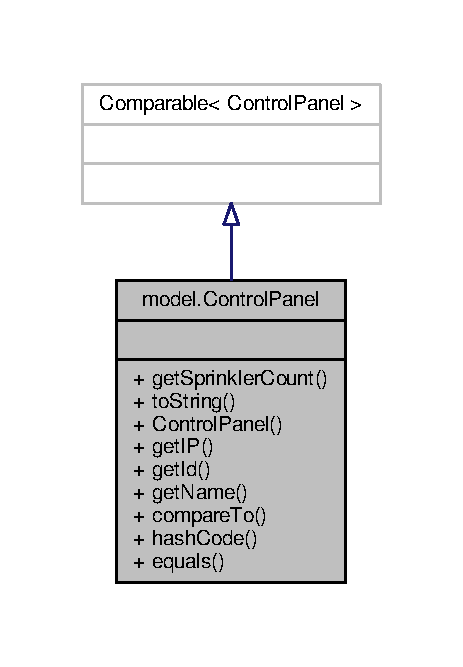
\includegraphics[width=222pt]{classmodel_1_1ControlPanel__inherit__graph}
\end{center}
\end{figure}


Collaboration diagram for model.\-Control\-Panel\-:\nopagebreak
\begin{figure}[H]
\begin{center}
\leavevmode
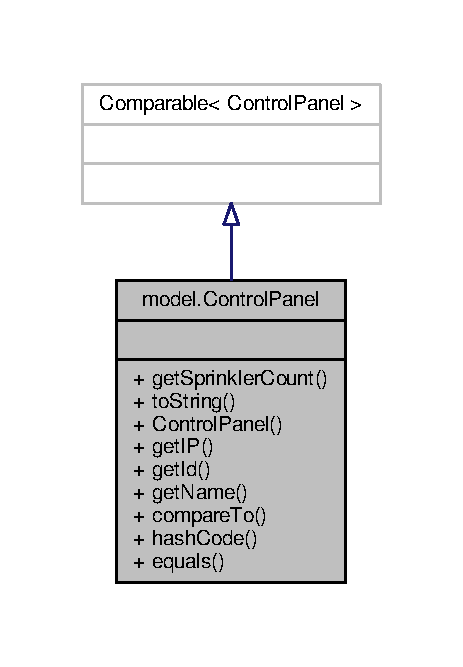
\includegraphics[width=222pt]{classmodel_1_1ControlPanel__coll__graph}
\end{center}
\end{figure}
\subsection*{Public Member Functions}
\begin{DoxyCompactItemize}
\item 
int \hyperlink{classmodel_1_1ControlPanel_af7dc341ae82b57608823abae7c64097e}{get\-Sprinkler\-Count} ()
\begin{DoxyCompactList}\small\item\em Gets count of Sprinklers. \end{DoxyCompactList}\item 
\hypertarget{classmodel_1_1ControlPanel_aa4272fa40dd552125416bd9c9349dd66}{String {\bfseries to\-String} ()}\label{classmodel_1_1ControlPanel_aa4272fa40dd552125416bd9c9349dd66}

\item 
\hyperlink{classmodel_1_1ControlPanel_a43731580310f63277399f974fef7f3ec}{Control\-Panel} (int id, String name, String host, int sprinkler\-Count)
\item 
String \hyperlink{classmodel_1_1ControlPanel_a9bfa823323b666a53ff799d00c6e2919}{get\-I\-P} ()
\item 
int \hyperlink{classmodel_1_1ControlPanel_a2aa5b49b94ed6d3e26142ccb695586b9}{get\-Id} ()
\item 
String \hyperlink{classmodel_1_1ControlPanel_a35bf96becebe31e08e827614b4ac230a}{get\-Name} ()
\item 
\hypertarget{classmodel_1_1ControlPanel_afec852bfbbe6280b16f1da4dfcd6241c}{int {\bfseries compare\-To} (\hyperlink{classmodel_1_1ControlPanel}{Control\-Panel} other)}\label{classmodel_1_1ControlPanel_afec852bfbbe6280b16f1da4dfcd6241c}

\item 
\hypertarget{classmodel_1_1ControlPanel_a7d46efd572aa30bec5daf492130f99a2}{int {\bfseries hash\-Code} ()}\label{classmodel_1_1ControlPanel_a7d46efd572aa30bec5daf492130f99a2}

\item 
\hypertarget{classmodel_1_1ControlPanel_adf64cd0f8b0529baa0a0bcc5542a3d29}{boolean {\bfseries equals} (Object obj)}\label{classmodel_1_1ControlPanel_adf64cd0f8b0529baa0a0bcc5542a3d29}

\end{DoxyCompactItemize}


\subsection{Detailed Description}
\begin{DoxyAuthor}{Author}
palmyman 
\end{DoxyAuthor}


\subsection{Constructor \& Destructor Documentation}
\hypertarget{classmodel_1_1ControlPanel_a43731580310f63277399f974fef7f3ec}{\index{model\-::\-Control\-Panel@{model\-::\-Control\-Panel}!Control\-Panel@{Control\-Panel}}
\index{Control\-Panel@{Control\-Panel}!model::ControlPanel@{model\-::\-Control\-Panel}}
\subsubsection[{Control\-Panel}]{\setlength{\rightskip}{0pt plus 5cm}model.\-Control\-Panel.\-Control\-Panel (
\begin{DoxyParamCaption}
\item[{int}]{id, }
\item[{String}]{name, }
\item[{String}]{host, }
\item[{int}]{sprinkler\-Count}
\end{DoxyParamCaption}
)\hspace{0.3cm}{\ttfamily [inline]}}}\label{classmodel_1_1ControlPanel_a43731580310f63277399f974fef7f3ec}

\begin{DoxyParams}{Parameters}
{\em id} & \\
\hline
{\em name} & \\
\hline
{\em host} & \\
\hline
{\em sprinkler\-Count} & \\
\hline
\end{DoxyParams}


\subsection{Member Function Documentation}
\hypertarget{classmodel_1_1ControlPanel_a2aa5b49b94ed6d3e26142ccb695586b9}{\index{model\-::\-Control\-Panel@{model\-::\-Control\-Panel}!get\-Id@{get\-Id}}
\index{get\-Id@{get\-Id}!model::ControlPanel@{model\-::\-Control\-Panel}}
\subsubsection[{get\-Id}]{\setlength{\rightskip}{0pt plus 5cm}int model.\-Control\-Panel.\-get\-Id (
\begin{DoxyParamCaption}
{}
\end{DoxyParamCaption}
)\hspace{0.3cm}{\ttfamily [inline]}}}\label{classmodel_1_1ControlPanel_a2aa5b49b94ed6d3e26142ccb695586b9}
\begin{DoxyReturn}{Returns}

\end{DoxyReturn}
\hypertarget{classmodel_1_1ControlPanel_a9bfa823323b666a53ff799d00c6e2919}{\index{model\-::\-Control\-Panel@{model\-::\-Control\-Panel}!get\-I\-P@{get\-I\-P}}
\index{get\-I\-P@{get\-I\-P}!model::ControlPanel@{model\-::\-Control\-Panel}}
\subsubsection[{get\-I\-P}]{\setlength{\rightskip}{0pt plus 5cm}String model.\-Control\-Panel.\-get\-I\-P (
\begin{DoxyParamCaption}
{}
\end{DoxyParamCaption}
)\hspace{0.3cm}{\ttfamily [inline]}}}\label{classmodel_1_1ControlPanel_a9bfa823323b666a53ff799d00c6e2919}
\begin{DoxyReturn}{Returns}

\end{DoxyReturn}
\hypertarget{classmodel_1_1ControlPanel_a35bf96becebe31e08e827614b4ac230a}{\index{model\-::\-Control\-Panel@{model\-::\-Control\-Panel}!get\-Name@{get\-Name}}
\index{get\-Name@{get\-Name}!model::ControlPanel@{model\-::\-Control\-Panel}}
\subsubsection[{get\-Name}]{\setlength{\rightskip}{0pt plus 5cm}String model.\-Control\-Panel.\-get\-Name (
\begin{DoxyParamCaption}
{}
\end{DoxyParamCaption}
)\hspace{0.3cm}{\ttfamily [inline]}}}\label{classmodel_1_1ControlPanel_a35bf96becebe31e08e827614b4ac230a}
\begin{DoxyReturn}{Returns}

\end{DoxyReturn}
\hypertarget{classmodel_1_1ControlPanel_af7dc341ae82b57608823abae7c64097e}{\index{model\-::\-Control\-Panel@{model\-::\-Control\-Panel}!get\-Sprinkler\-Count@{get\-Sprinkler\-Count}}
\index{get\-Sprinkler\-Count@{get\-Sprinkler\-Count}!model::ControlPanel@{model\-::\-Control\-Panel}}
\subsubsection[{get\-Sprinkler\-Count}]{\setlength{\rightskip}{0pt plus 5cm}int model.\-Control\-Panel.\-get\-Sprinkler\-Count (
\begin{DoxyParamCaption}
{}
\end{DoxyParamCaption}
)\hspace{0.3cm}{\ttfamily [inline]}}}\label{classmodel_1_1ControlPanel_af7dc341ae82b57608823abae7c64097e}


Gets count of Sprinklers. 

\begin{DoxyReturn}{Returns}
count of Sprinklers 
\end{DoxyReturn}


The documentation for this class was generated from the following file\-:\begin{DoxyCompactItemize}
\item 
src/model/Control\-Panel.\-java\end{DoxyCompactItemize}

\hypertarget{classdatabase_1_1ControlPanelDAO}{\section{database.\-Control\-Panel\-D\-A\-O Class Reference}
\label{classdatabase_1_1ControlPanelDAO}\index{database.\-Control\-Panel\-D\-A\-O@{database.\-Control\-Panel\-D\-A\-O}}
}


\hyperlink{classdatabase_1_1ControlPanelDAO}{Control\-Panel\-D\-A\-O} -\/ Data access object for Control\-Panel  




Inheritance diagram for database.\-Control\-Panel\-D\-A\-O\-:\nopagebreak
\begin{figure}[H]
\begin{center}
\leavevmode
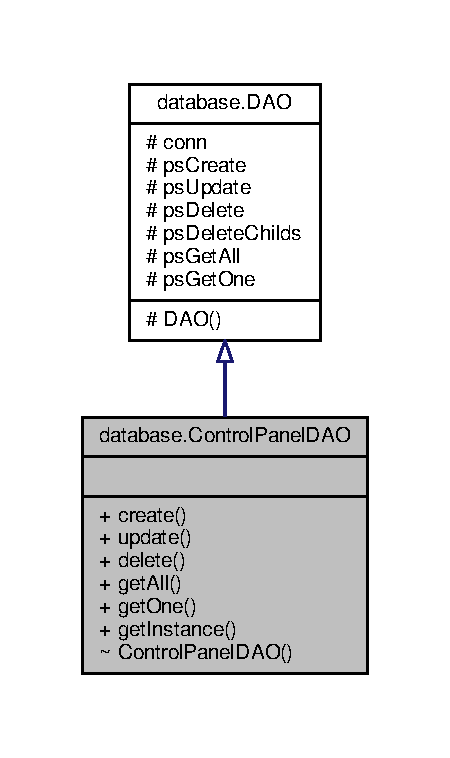
\includegraphics[width=216pt]{classdatabase_1_1ControlPanelDAO__inherit__graph}
\end{center}
\end{figure}


Collaboration diagram for database.\-Control\-Panel\-D\-A\-O\-:\nopagebreak
\begin{figure}[H]
\begin{center}
\leavevmode
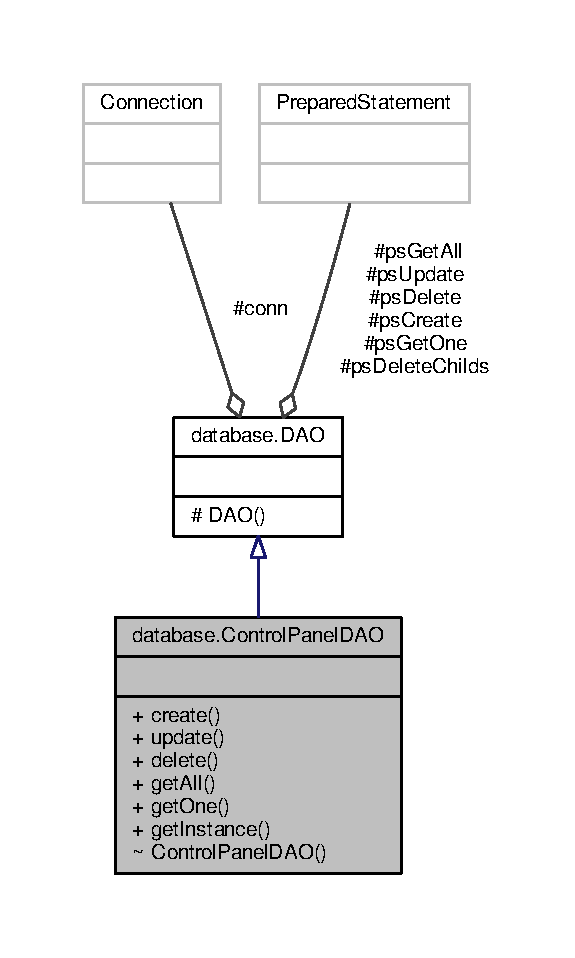
\includegraphics[width=276pt]{classdatabase_1_1ControlPanelDAO__coll__graph}
\end{center}
\end{figure}
\subsection*{Public Member Functions}
\begin{DoxyCompactItemize}
\item 
void \hyperlink{classdatabase_1_1ControlPanelDAO_a26bf174c6843577170698637da59c42b}{create} (\hyperlink{classmodel_1_1ControlPanel}{Control\-Panel} panel)  throws S\-Q\-L\-Exception 
\begin{DoxyCompactList}\small\item\em Persists new Control\-Panel. \end{DoxyCompactList}\item 
void \hyperlink{classdatabase_1_1ControlPanelDAO_a32dd5b996d60643f82b8dcccfd80c189}{update} (\hyperlink{classmodel_1_1ControlPanel}{Control\-Panel} panel)  throws S\-Q\-L\-Exception 
\begin{DoxyCompactList}\small\item\em Updates Control\-Panel. \end{DoxyCompactList}\item 
void \hyperlink{classdatabase_1_1ControlPanelDAO_a1a4a1168f864952c013e3dfe19f2822e}{delete} (\hyperlink{classmodel_1_1ControlPanel}{Control\-Panel} panel)  throws S\-Q\-L\-Exception 
\begin{DoxyCompactList}\small\item\em Deletes Control\-Panel. \end{DoxyCompactList}\item 
Collection$<$ \hyperlink{classmodel_1_1ControlPanel}{Control\-Panel} $>$ \hyperlink{classdatabase_1_1ControlPanelDAO_a0eb46ac26e7539cd6a4c8053807e1e49}{get\-All} ()  throws S\-Q\-L\-Exception 
\begin{DoxyCompactList}\small\item\em Gets all Control\-Panel records from database. \end{DoxyCompactList}\item 
\hyperlink{classmodel_1_1ControlPanel}{Control\-Panel} \hyperlink{classdatabase_1_1ControlPanelDAO_ab7297ef5c4058a1e6a78928a451eed7f}{get\-One} (int id)  throws S\-Q\-L\-Exception 
\begin{DoxyCompactList}\small\item\em Gets one Control\-Panel from database by I\-D. \end{DoxyCompactList}\end{DoxyCompactItemize}
\subsection*{Static Public Member Functions}
\begin{DoxyCompactItemize}
\item 
static \hyperlink{classdatabase_1_1ControlPanelDAO}{Control\-Panel\-D\-A\-O} \hyperlink{classdatabase_1_1ControlPanelDAO_ae8576a0313a13f04339df4654d2f76af}{get\-Instance} ()
\begin{DoxyCompactList}\small\item\em Instance getter. \end{DoxyCompactList}\end{DoxyCompactItemize}
\subsection*{Additional Inherited Members}


\subsection{Detailed Description}
\hyperlink{classdatabase_1_1ControlPanelDAO}{Control\-Panel\-D\-A\-O} -\/ Data access object for Control\-Panel 

\begin{DoxyAuthor}{Author}
palmyman 
\end{DoxyAuthor}


\subsection{Member Function Documentation}
\hypertarget{classdatabase_1_1ControlPanelDAO_a26bf174c6843577170698637da59c42b}{\index{database\-::\-Control\-Panel\-D\-A\-O@{database\-::\-Control\-Panel\-D\-A\-O}!create@{create}}
\index{create@{create}!database::ControlPanelDAO@{database\-::\-Control\-Panel\-D\-A\-O}}
\subsubsection[{create}]{\setlength{\rightskip}{0pt plus 5cm}void database.\-Control\-Panel\-D\-A\-O.\-create (
\begin{DoxyParamCaption}
\item[{{\bf Control\-Panel}}]{panel}
\end{DoxyParamCaption}
) throws S\-Q\-L\-Exception\hspace{0.3cm}{\ttfamily [inline]}}}\label{classdatabase_1_1ControlPanelDAO_a26bf174c6843577170698637da59c42b}


Persists new Control\-Panel. 


\begin{DoxyParams}{Parameters}
{\em panel} & Control\-Panel to persist \\
\hline
\end{DoxyParams}

\begin{DoxyExceptions}{Exceptions}
{\em S\-Q\-L\-Exception} & \\
\hline
\end{DoxyExceptions}
\hypertarget{classdatabase_1_1ControlPanelDAO_a1a4a1168f864952c013e3dfe19f2822e}{\index{database\-::\-Control\-Panel\-D\-A\-O@{database\-::\-Control\-Panel\-D\-A\-O}!delete@{delete}}
\index{delete@{delete}!database::ControlPanelDAO@{database\-::\-Control\-Panel\-D\-A\-O}}
\subsubsection[{delete}]{\setlength{\rightskip}{0pt plus 5cm}void database.\-Control\-Panel\-D\-A\-O.\-delete (
\begin{DoxyParamCaption}
\item[{{\bf Control\-Panel}}]{panel}
\end{DoxyParamCaption}
) throws S\-Q\-L\-Exception\hspace{0.3cm}{\ttfamily [inline]}}}\label{classdatabase_1_1ControlPanelDAO_a1a4a1168f864952c013e3dfe19f2822e}


Deletes Control\-Panel. 


\begin{DoxyParams}{Parameters}
{\em panel} & Control\-Panel to delete \\
\hline
\end{DoxyParams}

\begin{DoxyExceptions}{Exceptions}
{\em S\-Q\-L\-Exception} & \\
\hline
\end{DoxyExceptions}
\hypertarget{classdatabase_1_1ControlPanelDAO_a0eb46ac26e7539cd6a4c8053807e1e49}{\index{database\-::\-Control\-Panel\-D\-A\-O@{database\-::\-Control\-Panel\-D\-A\-O}!get\-All@{get\-All}}
\index{get\-All@{get\-All}!database::ControlPanelDAO@{database\-::\-Control\-Panel\-D\-A\-O}}
\subsubsection[{get\-All}]{\setlength{\rightskip}{0pt plus 5cm}Collection$<${\bf Control\-Panel}$>$ database.\-Control\-Panel\-D\-A\-O.\-get\-All (
\begin{DoxyParamCaption}
{}
\end{DoxyParamCaption}
) throws S\-Q\-L\-Exception\hspace{0.3cm}{\ttfamily [inline]}}}\label{classdatabase_1_1ControlPanelDAO_a0eb46ac26e7539cd6a4c8053807e1e49}


Gets all Control\-Panel records from database. 

\begin{DoxyReturn}{Returns}
Set of all Control\-Panels from database 
\end{DoxyReturn}

\begin{DoxyExceptions}{Exceptions}
{\em S\-Q\-L\-Exception} & \\
\hline
\end{DoxyExceptions}
\hypertarget{classdatabase_1_1ControlPanelDAO_ae8576a0313a13f04339df4654d2f76af}{\index{database\-::\-Control\-Panel\-D\-A\-O@{database\-::\-Control\-Panel\-D\-A\-O}!get\-Instance@{get\-Instance}}
\index{get\-Instance@{get\-Instance}!database::ControlPanelDAO@{database\-::\-Control\-Panel\-D\-A\-O}}
\subsubsection[{get\-Instance}]{\setlength{\rightskip}{0pt plus 5cm}static {\bf Control\-Panel\-D\-A\-O} database.\-Control\-Panel\-D\-A\-O.\-get\-Instance (
\begin{DoxyParamCaption}
{}
\end{DoxyParamCaption}
)\hspace{0.3cm}{\ttfamily [inline]}, {\ttfamily [static]}}}\label{classdatabase_1_1ControlPanelDAO_ae8576a0313a13f04339df4654d2f76af}


Instance getter. 

\begin{DoxyReturn}{Returns}
instance 
\end{DoxyReturn}
\hypertarget{classdatabase_1_1ControlPanelDAO_ab7297ef5c4058a1e6a78928a451eed7f}{\index{database\-::\-Control\-Panel\-D\-A\-O@{database\-::\-Control\-Panel\-D\-A\-O}!get\-One@{get\-One}}
\index{get\-One@{get\-One}!database::ControlPanelDAO@{database\-::\-Control\-Panel\-D\-A\-O}}
\subsubsection[{get\-One}]{\setlength{\rightskip}{0pt plus 5cm}{\bf Control\-Panel} database.\-Control\-Panel\-D\-A\-O.\-get\-One (
\begin{DoxyParamCaption}
\item[{int}]{id}
\end{DoxyParamCaption}
) throws S\-Q\-L\-Exception\hspace{0.3cm}{\ttfamily [inline]}}}\label{classdatabase_1_1ControlPanelDAO_ab7297ef5c4058a1e6a78928a451eed7f}


Gets one Control\-Panel from database by I\-D. 


\begin{DoxyParams}{Parameters}
{\em id} & I\-D of Control\-Panel \\
\hline
\end{DoxyParams}
\begin{DoxyReturn}{Returns}
Control\-Panel if found, else returns null 
\end{DoxyReturn}

\begin{DoxyExceptions}{Exceptions}
{\em S\-Q\-L\-Exception} & \\
\hline
\end{DoxyExceptions}
\hypertarget{classdatabase_1_1ControlPanelDAO_a32dd5b996d60643f82b8dcccfd80c189}{\index{database\-::\-Control\-Panel\-D\-A\-O@{database\-::\-Control\-Panel\-D\-A\-O}!update@{update}}
\index{update@{update}!database::ControlPanelDAO@{database\-::\-Control\-Panel\-D\-A\-O}}
\subsubsection[{update}]{\setlength{\rightskip}{0pt plus 5cm}void database.\-Control\-Panel\-D\-A\-O.\-update (
\begin{DoxyParamCaption}
\item[{{\bf Control\-Panel}}]{panel}
\end{DoxyParamCaption}
) throws S\-Q\-L\-Exception\hspace{0.3cm}{\ttfamily [inline]}}}\label{classdatabase_1_1ControlPanelDAO_a32dd5b996d60643f82b8dcccfd80c189}


Updates Control\-Panel. 


\begin{DoxyParams}{Parameters}
{\em panel} & Control\-Panel to update \\
\hline
\end{DoxyParams}

\begin{DoxyExceptions}{Exceptions}
{\em S\-Q\-L\-Exception} & \\
\hline
\end{DoxyExceptions}


The documentation for this class was generated from the following file\-:\begin{DoxyCompactItemize}
\item 
src/database/Control\-Panel\-D\-A\-O.\-java\end{DoxyCompactItemize}

\hypertarget{classdatabase_1_1DAO}{\section{database.\-D\-A\-O Class Reference}
\label{classdatabase_1_1DAO}\index{database.\-D\-A\-O@{database.\-D\-A\-O}}
}


\hyperlink{classdatabase_1_1DAO}{D\-A\-O} -\/ Data access object  




Inheritance diagram for database.\-D\-A\-O\-:\nopagebreak
\begin{figure}[H]
\begin{center}
\leavevmode
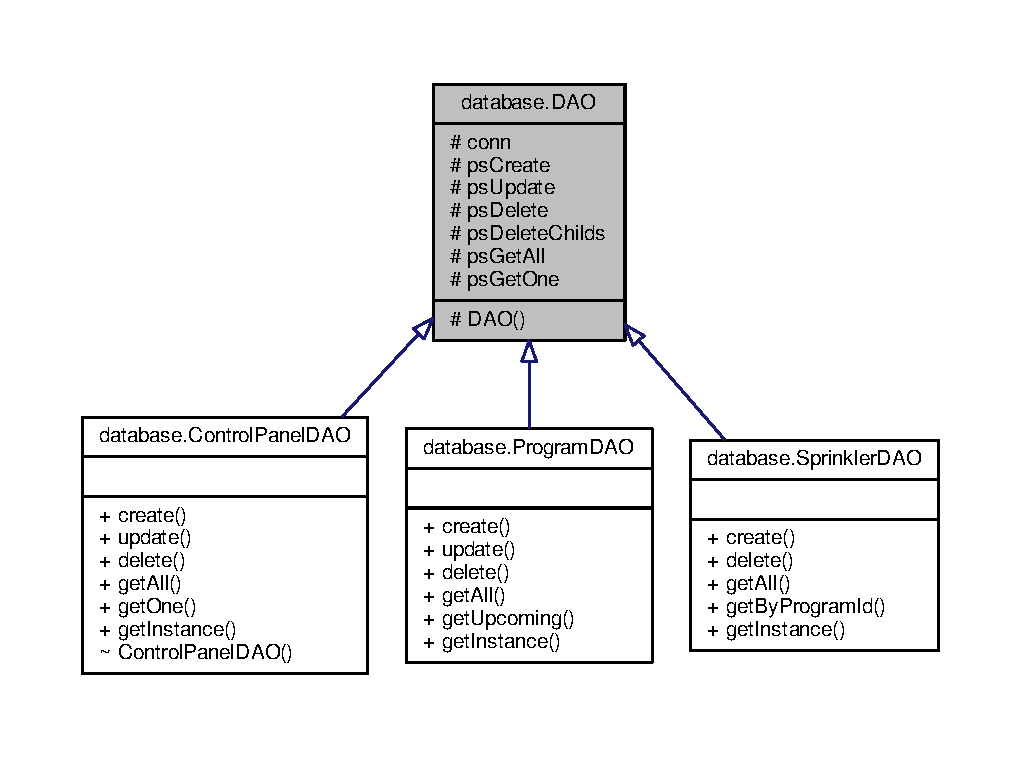
\includegraphics[width=350pt]{classdatabase_1_1DAO__inherit__graph}
\end{center}
\end{figure}


Collaboration diagram for database.\-D\-A\-O\-:\nopagebreak
\begin{figure}[H]
\begin{center}
\leavevmode
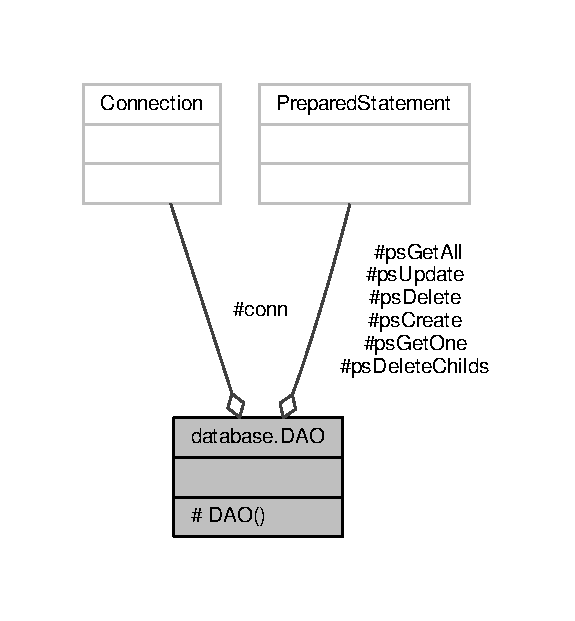
\includegraphics[width=276pt]{classdatabase_1_1DAO__coll__graph}
\end{center}
\end{figure}
\subsection*{Protected Member Functions}
\begin{DoxyCompactItemize}
\item 
\hyperlink{classdatabase_1_1DAO_acb47f8f2c2185ebede743cc5fd6d3449}{D\-A\-O} ()
\begin{DoxyCompactList}\small\item\em \hyperlink{classdatabase_1_1DAO}{D\-A\-O} constructor. \end{DoxyCompactList}\end{DoxyCompactItemize}
\subsection*{Protected Attributes}
\begin{DoxyCompactItemize}
\item 
\hypertarget{classdatabase_1_1DAO_a8db8acaec4cf340eee4907a3b4fe8b60}{Connection \hyperlink{classdatabase_1_1DAO_a8db8acaec4cf340eee4907a3b4fe8b60}{conn}}\label{classdatabase_1_1DAO_a8db8acaec4cf340eee4907a3b4fe8b60}

\begin{DoxyCompactList}\small\item\em Connection to database. \end{DoxyCompactList}\item 
\hypertarget{classdatabase_1_1DAO_a1f02dc2793eb1fd62da5abfda09a0667}{Prepared\-Statement \hyperlink{classdatabase_1_1DAO_a1f02dc2793eb1fd62da5abfda09a0667}{ps\-Create}}\label{classdatabase_1_1DAO_a1f02dc2793eb1fd62da5abfda09a0667}

\begin{DoxyCompactList}\small\item\em Create prepared statement. \end{DoxyCompactList}\item 
\hypertarget{classdatabase_1_1DAO_a0ae3296c0df031e312507b1e435669a4}{Prepared\-Statement \hyperlink{classdatabase_1_1DAO_a0ae3296c0df031e312507b1e435669a4}{ps\-Update}}\label{classdatabase_1_1DAO_a0ae3296c0df031e312507b1e435669a4}

\begin{DoxyCompactList}\small\item\em Update prepared statement. \end{DoxyCompactList}\item 
\hypertarget{classdatabase_1_1DAO_a21fb0047b0095c65e924e14e44131a5a}{Prepared\-Statement \hyperlink{classdatabase_1_1DAO_a21fb0047b0095c65e924e14e44131a5a}{ps\-Delete}}\label{classdatabase_1_1DAO_a21fb0047b0095c65e924e14e44131a5a}

\begin{DoxyCompactList}\small\item\em Delete prepared statement. \end{DoxyCompactList}\item 
\hypertarget{classdatabase_1_1DAO_ac0f9df0f9e0f243dc38a3ade6511ad40}{Prepared\-Statement \hyperlink{classdatabase_1_1DAO_ac0f9df0f9e0f243dc38a3ade6511ad40}{ps\-Delete\-Childs}}\label{classdatabase_1_1DAO_ac0f9df0f9e0f243dc38a3ade6511ad40}

\begin{DoxyCompactList}\small\item\em Delete children prepared statement. \end{DoxyCompactList}\item 
\hypertarget{classdatabase_1_1DAO_a6d19d7a937d5b1a6ab9a48467ef04ec4}{Prepared\-Statement \hyperlink{classdatabase_1_1DAO_a6d19d7a937d5b1a6ab9a48467ef04ec4}{ps\-Get\-All}}\label{classdatabase_1_1DAO_a6d19d7a937d5b1a6ab9a48467ef04ec4}

\begin{DoxyCompactList}\small\item\em Get all prepared statement. \end{DoxyCompactList}\item 
\hypertarget{classdatabase_1_1DAO_a695bfa9f357dcd8a9f90e28fb6822a9b}{Prepared\-Statement \hyperlink{classdatabase_1_1DAO_a695bfa9f357dcd8a9f90e28fb6822a9b}{ps\-Get\-One}}\label{classdatabase_1_1DAO_a695bfa9f357dcd8a9f90e28fb6822a9b}

\begin{DoxyCompactList}\small\item\em Get one prepared statement. \end{DoxyCompactList}\end{DoxyCompactItemize}


\subsection{Detailed Description}
\hyperlink{classdatabase_1_1DAO}{D\-A\-O} -\/ Data access object 

\begin{DoxyAuthor}{Author}
palmyman\-This object is used to initialize and work with the database 
\end{DoxyAuthor}


\subsection{Constructor \& Destructor Documentation}
\hypertarget{classdatabase_1_1DAO_acb47f8f2c2185ebede743cc5fd6d3449}{\index{database\-::\-D\-A\-O@{database\-::\-D\-A\-O}!D\-A\-O@{D\-A\-O}}
\index{D\-A\-O@{D\-A\-O}!database::DAO@{database\-::\-D\-A\-O}}
\subsubsection[{D\-A\-O}]{\setlength{\rightskip}{0pt plus 5cm}database.\-D\-A\-O.\-D\-A\-O (
\begin{DoxyParamCaption}
{}
\end{DoxyParamCaption}
)\hspace{0.3cm}{\ttfamily [inline]}, {\ttfamily [protected]}}}\label{classdatabase_1_1DAO_acb47f8f2c2185ebede743cc5fd6d3449}


\hyperlink{classdatabase_1_1DAO}{D\-A\-O} constructor. 

Establishes connection to database. If the database is empty, will initialize tables with sample data. 

The documentation for this class was generated from the following file\-:\begin{DoxyCompactItemize}
\item 
src/database/D\-A\-O.\-java\end{DoxyCompactItemize}

\hypertarget{classgui_1_1MainFrame}{\section{gui.\-Main\-Frame Class Reference}
\label{classgui_1_1MainFrame}\index{gui.\-Main\-Frame@{gui.\-Main\-Frame}}
}


Inheritance diagram for gui.\-Main\-Frame\-:\nopagebreak
\begin{figure}[H]
\begin{center}
\leavevmode
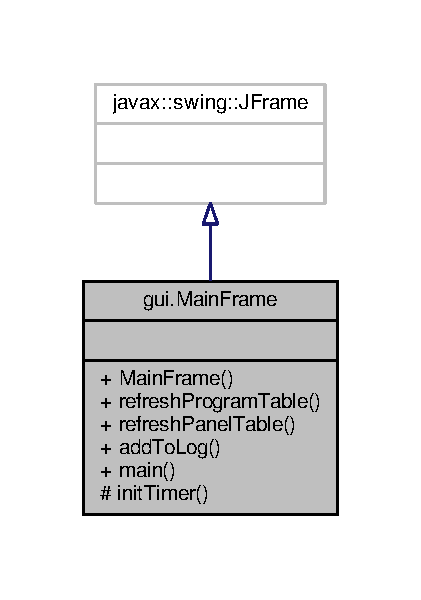
\includegraphics[width=202pt]{classgui_1_1MainFrame__inherit__graph}
\end{center}
\end{figure}


Collaboration diagram for gui.\-Main\-Frame\-:\nopagebreak
\begin{figure}[H]
\begin{center}
\leavevmode
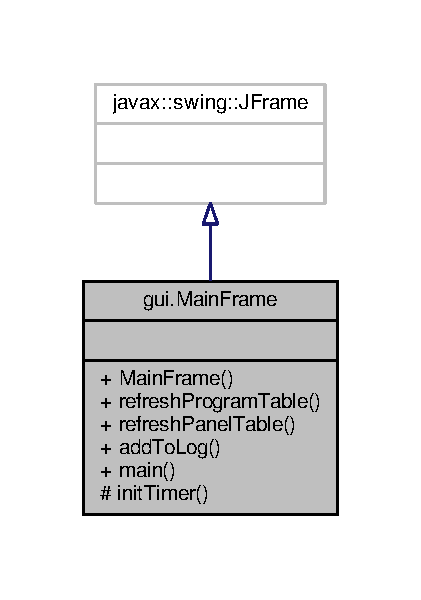
\includegraphics[width=202pt]{classgui_1_1MainFrame__coll__graph}
\end{center}
\end{figure}
\subsection*{Public Member Functions}
\begin{DoxyCompactItemize}
\item 
\hypertarget{classgui_1_1MainFrame_aaeeb6a0f50e5e5bddfa7f05d3871e9ec}{\hyperlink{classgui_1_1MainFrame_aaeeb6a0f50e5e5bddfa7f05d3871e9ec}{Main\-Frame} ()}\label{classgui_1_1MainFrame_aaeeb6a0f50e5e5bddfa7f05d3871e9ec}

\begin{DoxyCompactList}\small\item\em Creates new form \hyperlink{classgui_1_1MainFrame}{Main\-Frame}. \end{DoxyCompactList}\item 
\hypertarget{classgui_1_1MainFrame_a80f02b2b3a38e33da6a5cf95cf90dfa7}{void {\bfseries refresh\-Program\-Table} ()}\label{classgui_1_1MainFrame_a80f02b2b3a38e33da6a5cf95cf90dfa7}

\item 
\hypertarget{classgui_1_1MainFrame_aa191c6f403de836ce1818821026a6a1f}{void {\bfseries refresh\-Panel\-Table} ()}\label{classgui_1_1MainFrame_aa191c6f403de836ce1818821026a6a1f}

\item 
\hypertarget{classgui_1_1MainFrame_a3ff1c92e306a00fe2362a27f0e38d0ed}{void {\bfseries add\-To\-Log} (String text)}\label{classgui_1_1MainFrame_a3ff1c92e306a00fe2362a27f0e38d0ed}

\end{DoxyCompactItemize}
\subsection*{Static Public Member Functions}
\begin{DoxyCompactItemize}
\item 
static void \hyperlink{classgui_1_1MainFrame_a9426bc550d35eaa70ea8c78ff18dae56}{main} (String args\mbox{[}$\,$\mbox{]})
\end{DoxyCompactItemize}
\subsection*{Protected Member Functions}
\begin{DoxyCompactItemize}
\item 
\hypertarget{classgui_1_1MainFrame_a02cdeab719249c5c7de74f74d1eabf2b}{void {\bfseries init\-Timer} ()}\label{classgui_1_1MainFrame_a02cdeab719249c5c7de74f74d1eabf2b}

\end{DoxyCompactItemize}


\subsection{Detailed Description}
\begin{DoxyAuthor}{Author}
palmyman 
\end{DoxyAuthor}


\subsection{Member Function Documentation}
\hypertarget{classgui_1_1MainFrame_a9426bc550d35eaa70ea8c78ff18dae56}{\index{gui\-::\-Main\-Frame@{gui\-::\-Main\-Frame}!main@{main}}
\index{main@{main}!gui::MainFrame@{gui\-::\-Main\-Frame}}
\subsubsection[{main}]{\setlength{\rightskip}{0pt plus 5cm}static void gui.\-Main\-Frame.\-main (
\begin{DoxyParamCaption}
\item[{String}]{args\mbox{[}$\,$\mbox{]}}
\end{DoxyParamCaption}
)\hspace{0.3cm}{\ttfamily [inline]}, {\ttfamily [static]}}}\label{classgui_1_1MainFrame_a9426bc550d35eaa70ea8c78ff18dae56}

\begin{DoxyParams}{Parameters}
{\em args} & the command line arguments \\
\hline
\end{DoxyParams}


The documentation for this class was generated from the following file\-:\begin{DoxyCompactItemize}
\item 
src/gui/Main\-Frame.\-java\end{DoxyCompactItemize}

\hypertarget{classgui_1_1NewPanelDialog}{\section{gui.\-New\-Panel\-Dialog Class Reference}
\label{classgui_1_1NewPanelDialog}\index{gui.\-New\-Panel\-Dialog@{gui.\-New\-Panel\-Dialog}}
}


Inheritance diagram for gui.\-New\-Panel\-Dialog\-:\nopagebreak
\begin{figure}[H]
\begin{center}
\leavevmode
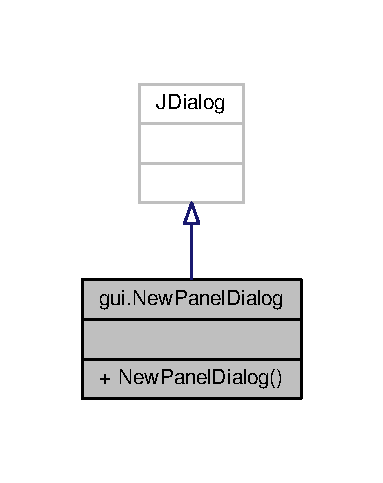
\includegraphics[width=184pt]{classgui_1_1NewPanelDialog__inherit__graph}
\end{center}
\end{figure}


Collaboration diagram for gui.\-New\-Panel\-Dialog\-:\nopagebreak
\begin{figure}[H]
\begin{center}
\leavevmode
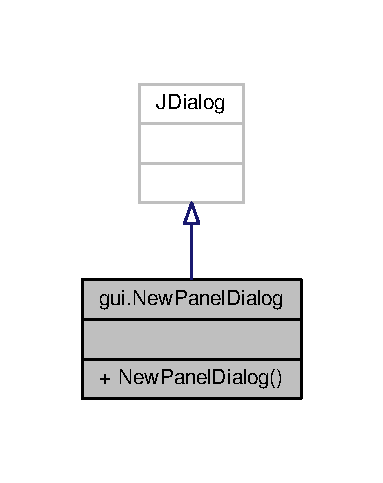
\includegraphics[width=184pt]{classgui_1_1NewPanelDialog__coll__graph}
\end{center}
\end{figure}
\subsection*{Public Member Functions}
\begin{DoxyCompactItemize}
\item 
\hypertarget{classgui_1_1NewPanelDialog_a325de0e08c74ba14c31c46d70320d369}{\hyperlink{classgui_1_1NewPanelDialog_a325de0e08c74ba14c31c46d70320d369}{New\-Panel\-Dialog} ()}\label{classgui_1_1NewPanelDialog_a325de0e08c74ba14c31c46d70320d369}

\begin{DoxyCompactList}\small\item\em Creates new form \hyperlink{classgui_1_1NewProgramDialog}{New\-Program\-Dialog}. \end{DoxyCompactList}\end{DoxyCompactItemize}


\subsection{Detailed Description}
\begin{DoxyAuthor}{Author}
palmyman 
\end{DoxyAuthor}


The documentation for this class was generated from the following file\-:\begin{DoxyCompactItemize}
\item 
src/gui/New\-Panel\-Dialog.\-java\end{DoxyCompactItemize}

\hypertarget{classgui_1_1NewProgramDialog}{\section{gui.\-New\-Program\-Dialog Class Reference}
\label{classgui_1_1NewProgramDialog}\index{gui.\-New\-Program\-Dialog@{gui.\-New\-Program\-Dialog}}
}


Inheritance diagram for gui.\-New\-Program\-Dialog\-:\nopagebreak
\begin{figure}[H]
\begin{center}
\leavevmode
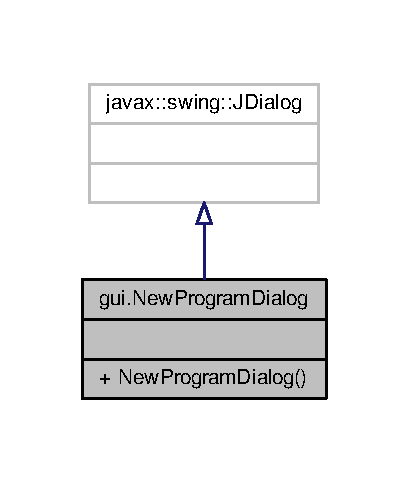
\includegraphics[width=196pt]{classgui_1_1NewProgramDialog__inherit__graph}
\end{center}
\end{figure}


Collaboration diagram for gui.\-New\-Program\-Dialog\-:\nopagebreak
\begin{figure}[H]
\begin{center}
\leavevmode
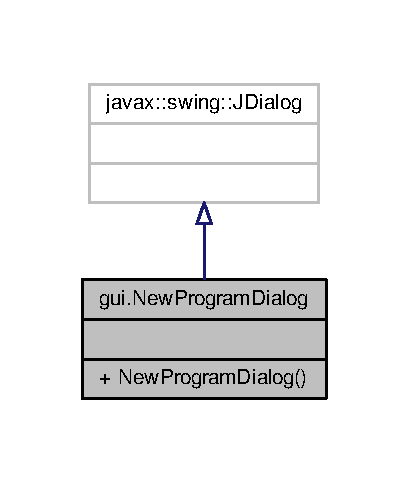
\includegraphics[width=196pt]{classgui_1_1NewProgramDialog__coll__graph}
\end{center}
\end{figure}
\subsection*{Public Member Functions}
\begin{DoxyCompactItemize}
\item 
\hypertarget{classgui_1_1NewProgramDialog_a8d544e87a6426218e20fca917dcfe7d8}{\hyperlink{classgui_1_1NewProgramDialog_a8d544e87a6426218e20fca917dcfe7d8}{New\-Program\-Dialog} ()}\label{classgui_1_1NewProgramDialog_a8d544e87a6426218e20fca917dcfe7d8}

\begin{DoxyCompactList}\small\item\em Creates new form \hyperlink{classgui_1_1NewProgramDialog}{New\-Program\-Dialog}. \end{DoxyCompactList}\end{DoxyCompactItemize}


\subsection{Detailed Description}
\begin{DoxyAuthor}{Author}
palmyman 
\end{DoxyAuthor}


The documentation for this class was generated from the following file\-:\begin{DoxyCompactItemize}
\item 
src/gui/New\-Program\-Dialog.\-java\end{DoxyCompactItemize}

\hypertarget{classgui_1_1PanelEditorDialog}{\section{gui.\-Panel\-Editor\-Dialog Class Reference}
\label{classgui_1_1PanelEditorDialog}\index{gui.\-Panel\-Editor\-Dialog@{gui.\-Panel\-Editor\-Dialog}}
}


Inheritance diagram for gui.\-Panel\-Editor\-Dialog\-:\nopagebreak
\begin{figure}[H]
\begin{center}
\leavevmode
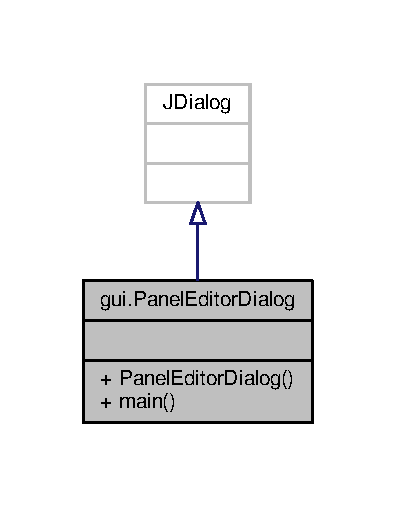
\includegraphics[width=190pt]{classgui_1_1PanelEditorDialog__inherit__graph}
\end{center}
\end{figure}


Collaboration diagram for gui.\-Panel\-Editor\-Dialog\-:\nopagebreak
\begin{figure}[H]
\begin{center}
\leavevmode
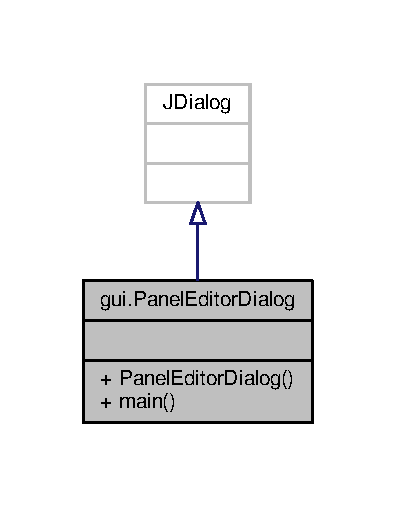
\includegraphics[width=190pt]{classgui_1_1PanelEditorDialog__coll__graph}
\end{center}
\end{figure}
\subsection*{Public Member Functions}
\begin{DoxyCompactItemize}
\item 
\hypertarget{classgui_1_1PanelEditorDialog_a28c7b8ddc1397ceb3f876db530f56b5d}{\hyperlink{classgui_1_1PanelEditorDialog_a28c7b8ddc1397ceb3f876db530f56b5d}{Panel\-Editor\-Dialog} ()}\label{classgui_1_1PanelEditorDialog_a28c7b8ddc1397ceb3f876db530f56b5d}

\begin{DoxyCompactList}\small\item\em Creates new form \hyperlink{classgui_1_1NewProgramDialog}{New\-Program\-Dialog}. \end{DoxyCompactList}\end{DoxyCompactItemize}
\subsection*{Static Public Member Functions}
\begin{DoxyCompactItemize}
\item 
static void \hyperlink{classgui_1_1PanelEditorDialog_a42df09b48f2713499bc3102a0aa8e210}{main} (String args\mbox{[}$\,$\mbox{]})
\end{DoxyCompactItemize}


\subsection{Detailed Description}
\begin{DoxyAuthor}{Author}
palmyman 
\end{DoxyAuthor}


\subsection{Member Function Documentation}
\hypertarget{classgui_1_1PanelEditorDialog_a42df09b48f2713499bc3102a0aa8e210}{\index{gui\-::\-Panel\-Editor\-Dialog@{gui\-::\-Panel\-Editor\-Dialog}!main@{main}}
\index{main@{main}!gui::PanelEditorDialog@{gui\-::\-Panel\-Editor\-Dialog}}
\subsubsection[{main}]{\setlength{\rightskip}{0pt plus 5cm}static void gui.\-Panel\-Editor\-Dialog.\-main (
\begin{DoxyParamCaption}
\item[{String}]{args\mbox{[}$\,$\mbox{]}}
\end{DoxyParamCaption}
)\hspace{0.3cm}{\ttfamily [inline]}, {\ttfamily [static]}}}\label{classgui_1_1PanelEditorDialog_a42df09b48f2713499bc3102a0aa8e210}

\begin{DoxyParams}{Parameters}
{\em args} & the command line arguments \\
\hline
\end{DoxyParams}


The documentation for this class was generated from the following file\-:\begin{DoxyCompactItemize}
\item 
src/gui/Panel\-Editor\-Dialog.\-java\end{DoxyCompactItemize}

\hypertarget{classmodel_1_1Program}{\section{model.\-Program Class Reference}
\label{classmodel_1_1Program}\index{model.\-Program@{model.\-Program}}
}


Inheritance diagram for model.\-Program\-:\nopagebreak
\begin{figure}[H]
\begin{center}
\leavevmode
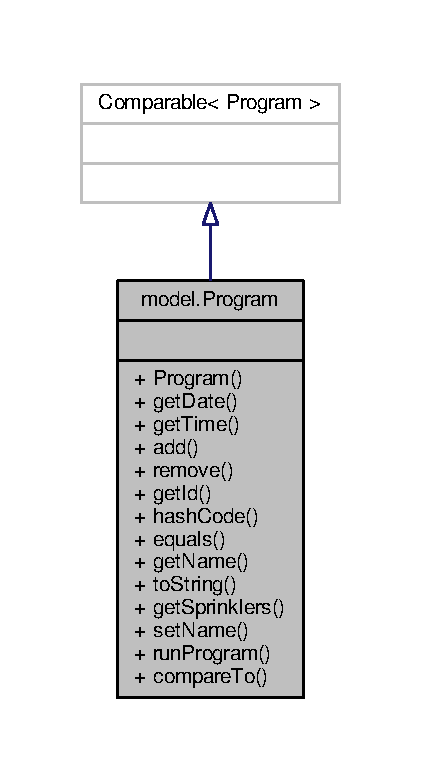
\includegraphics[width=202pt]{classmodel_1_1Program__inherit__graph}
\end{center}
\end{figure}


Collaboration diagram for model.\-Program\-:\nopagebreak
\begin{figure}[H]
\begin{center}
\leavevmode
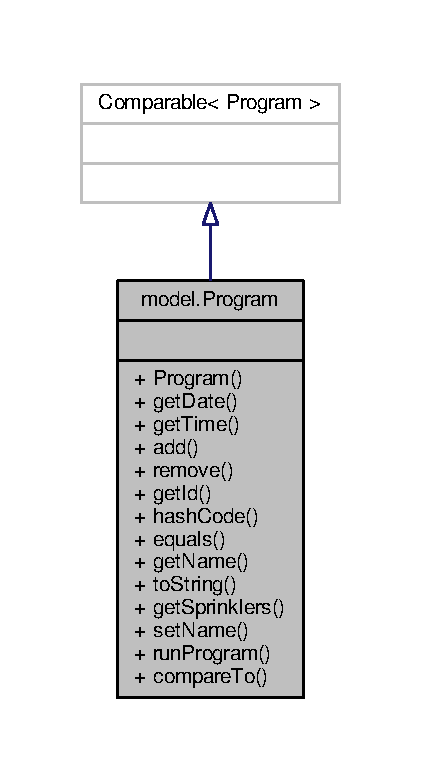
\includegraphics[width=202pt]{classmodel_1_1Program__coll__graph}
\end{center}
\end{figure}
\subsection*{Public Member Functions}
\begin{DoxyCompactItemize}
\item 
\hyperlink{classmodel_1_1Program_a6580a752cabd050b3e717b9f59257010}{Program} (int id, String name, Date date, Time time)
\item 
Date \hyperlink{classmodel_1_1Program_a07c6017d78569467ae4217ed87933498}{get\-Date} ()
\item 
Time \hyperlink{classmodel_1_1Program_a781bf64d5e29a0f857d0b9563c021aeb}{get\-Time} ()
\item 
boolean \hyperlink{classmodel_1_1Program_a5ee34c0bfa88ab0d6097091e710bdfd9}{add} (\hyperlink{classmodel_1_1TimedSprinkler}{Timed\-Sprinkler} item)
\item 
boolean \hyperlink{classmodel_1_1Program_a4ff329b2b132c99b350364e96ff33445}{remove} (\hyperlink{classmodel_1_1TimedSprinkler}{Timed\-Sprinkler} item)
\item 
int \hyperlink{classmodel_1_1Program_ad2341d28025213b84388cf5e3ec07fab}{get\-Id} ()
\item 
\hypertarget{classmodel_1_1Program_ae7e7a72285ff10446ce5b0b8193f576d}{int {\bfseries hash\-Code} ()}\label{classmodel_1_1Program_ae7e7a72285ff10446ce5b0b8193f576d}

\item 
boolean \hyperlink{classmodel_1_1Program_a9ae2c6573165fc32a5eba3bfa751bedc}{equals} (\hyperlink{classmodel_1_1Program}{Program} obj)
\item 
String \hyperlink{classmodel_1_1Program_a0a9a9037a0134dd5edc5daf037decce7}{get\-Name} ()
\item 
\hypertarget{classmodel_1_1Program_a1d12fed19095fc4c789716569abf4058}{String {\bfseries to\-String} ()}\label{classmodel_1_1Program_a1d12fed19095fc4c789716569abf4058}

\item 
Sorted\-Set$<$ \hyperlink{classmodel_1_1TimedSprinkler}{Timed\-Sprinkler} $>$ \hyperlink{classmodel_1_1Program_a2a8ca42dce071c88963d1be77ac80a9a}{get\-Sprinklers} ()
\item 
void \hyperlink{classmodel_1_1Program_ac6c3431fe0d1cc2245fad3d77b34d4f4}{set\-Name} (String name)
\item 
void \hyperlink{classmodel_1_1Program_a49d0f7485f5012791fd56928acb473ed}{run\-Program} ()  throws Interrupted\-Exception 
\item 
\hypertarget{classmodel_1_1Program_ae5dfdf7cf531a0b5edc40d8f64683d70}{int {\bfseries compare\-To} (\hyperlink{classmodel_1_1Program}{Program} other)}\label{classmodel_1_1Program_ae5dfdf7cf531a0b5edc40d8f64683d70}

\end{DoxyCompactItemize}


\subsection{Detailed Description}
\begin{DoxyAuthor}{Author}
palmyman 
\end{DoxyAuthor}


\subsection{Constructor \& Destructor Documentation}
\hypertarget{classmodel_1_1Program_a6580a752cabd050b3e717b9f59257010}{\index{model\-::\-Program@{model\-::\-Program}!Program@{Program}}
\index{Program@{Program}!model::Program@{model\-::\-Program}}
\subsubsection[{Program}]{\setlength{\rightskip}{0pt plus 5cm}model.\-Program.\-Program (
\begin{DoxyParamCaption}
\item[{int}]{id, }
\item[{String}]{name, }
\item[{Date}]{date, }
\item[{Time}]{time}
\end{DoxyParamCaption}
)\hspace{0.3cm}{\ttfamily [inline]}}}\label{classmodel_1_1Program_a6580a752cabd050b3e717b9f59257010}

\begin{DoxyParams}{Parameters}
{\em id} & \\
\hline
{\em name} & \\
\hline
{\em date} & \\
\hline
{\em time} & \\
\hline
\end{DoxyParams}


\subsection{Member Function Documentation}
\hypertarget{classmodel_1_1Program_a5ee34c0bfa88ab0d6097091e710bdfd9}{\index{model\-::\-Program@{model\-::\-Program}!add@{add}}
\index{add@{add}!model::Program@{model\-::\-Program}}
\subsubsection[{add}]{\setlength{\rightskip}{0pt plus 5cm}boolean model.\-Program.\-add (
\begin{DoxyParamCaption}
\item[{{\bf Timed\-Sprinkler}}]{item}
\end{DoxyParamCaption}
)\hspace{0.3cm}{\ttfamily [inline]}}}\label{classmodel_1_1Program_a5ee34c0bfa88ab0d6097091e710bdfd9}

\begin{DoxyParams}{Parameters}
{\em item} & \\
\hline
\end{DoxyParams}
\begin{DoxyReturn}{Returns}

\end{DoxyReturn}
\hypertarget{classmodel_1_1Program_a9ae2c6573165fc32a5eba3bfa751bedc}{\index{model\-::\-Program@{model\-::\-Program}!equals@{equals}}
\index{equals@{equals}!model::Program@{model\-::\-Program}}
\subsubsection[{equals}]{\setlength{\rightskip}{0pt plus 5cm}boolean model.\-Program.\-equals (
\begin{DoxyParamCaption}
\item[{{\bf Program}}]{obj}
\end{DoxyParamCaption}
)\hspace{0.3cm}{\ttfamily [inline]}}}\label{classmodel_1_1Program_a9ae2c6573165fc32a5eba3bfa751bedc}

\begin{DoxyParams}{Parameters}
{\em obj} & \\
\hline
\end{DoxyParams}
\begin{DoxyReturn}{Returns}

\end{DoxyReturn}
\hypertarget{classmodel_1_1Program_a07c6017d78569467ae4217ed87933498}{\index{model\-::\-Program@{model\-::\-Program}!get\-Date@{get\-Date}}
\index{get\-Date@{get\-Date}!model::Program@{model\-::\-Program}}
\subsubsection[{get\-Date}]{\setlength{\rightskip}{0pt plus 5cm}Date model.\-Program.\-get\-Date (
\begin{DoxyParamCaption}
{}
\end{DoxyParamCaption}
)\hspace{0.3cm}{\ttfamily [inline]}}}\label{classmodel_1_1Program_a07c6017d78569467ae4217ed87933498}
\begin{DoxyReturn}{Returns}

\end{DoxyReturn}
\hypertarget{classmodel_1_1Program_ad2341d28025213b84388cf5e3ec07fab}{\index{model\-::\-Program@{model\-::\-Program}!get\-Id@{get\-Id}}
\index{get\-Id@{get\-Id}!model::Program@{model\-::\-Program}}
\subsubsection[{get\-Id}]{\setlength{\rightskip}{0pt plus 5cm}int model.\-Program.\-get\-Id (
\begin{DoxyParamCaption}
{}
\end{DoxyParamCaption}
)\hspace{0.3cm}{\ttfamily [inline]}}}\label{classmodel_1_1Program_ad2341d28025213b84388cf5e3ec07fab}
\begin{DoxyReturn}{Returns}

\end{DoxyReturn}
\hypertarget{classmodel_1_1Program_a0a9a9037a0134dd5edc5daf037decce7}{\index{model\-::\-Program@{model\-::\-Program}!get\-Name@{get\-Name}}
\index{get\-Name@{get\-Name}!model::Program@{model\-::\-Program}}
\subsubsection[{get\-Name}]{\setlength{\rightskip}{0pt plus 5cm}String model.\-Program.\-get\-Name (
\begin{DoxyParamCaption}
{}
\end{DoxyParamCaption}
)\hspace{0.3cm}{\ttfamily [inline]}}}\label{classmodel_1_1Program_a0a9a9037a0134dd5edc5daf037decce7}
\begin{DoxyReturn}{Returns}

\end{DoxyReturn}
\hypertarget{classmodel_1_1Program_a2a8ca42dce071c88963d1be77ac80a9a}{\index{model\-::\-Program@{model\-::\-Program}!get\-Sprinklers@{get\-Sprinklers}}
\index{get\-Sprinklers@{get\-Sprinklers}!model::Program@{model\-::\-Program}}
\subsubsection[{get\-Sprinklers}]{\setlength{\rightskip}{0pt plus 5cm}Sorted\-Set$<${\bf Timed\-Sprinkler}$>$ model.\-Program.\-get\-Sprinklers (
\begin{DoxyParamCaption}
{}
\end{DoxyParamCaption}
)\hspace{0.3cm}{\ttfamily [inline]}}}\label{classmodel_1_1Program_a2a8ca42dce071c88963d1be77ac80a9a}
\begin{DoxyReturn}{Returns}

\end{DoxyReturn}
\hypertarget{classmodel_1_1Program_a781bf64d5e29a0f857d0b9563c021aeb}{\index{model\-::\-Program@{model\-::\-Program}!get\-Time@{get\-Time}}
\index{get\-Time@{get\-Time}!model::Program@{model\-::\-Program}}
\subsubsection[{get\-Time}]{\setlength{\rightskip}{0pt plus 5cm}Time model.\-Program.\-get\-Time (
\begin{DoxyParamCaption}
{}
\end{DoxyParamCaption}
)\hspace{0.3cm}{\ttfamily [inline]}}}\label{classmodel_1_1Program_a781bf64d5e29a0f857d0b9563c021aeb}
\begin{DoxyReturn}{Returns}

\end{DoxyReturn}
\hypertarget{classmodel_1_1Program_a4ff329b2b132c99b350364e96ff33445}{\index{model\-::\-Program@{model\-::\-Program}!remove@{remove}}
\index{remove@{remove}!model::Program@{model\-::\-Program}}
\subsubsection[{remove}]{\setlength{\rightskip}{0pt plus 5cm}boolean model.\-Program.\-remove (
\begin{DoxyParamCaption}
\item[{{\bf Timed\-Sprinkler}}]{item}
\end{DoxyParamCaption}
)\hspace{0.3cm}{\ttfamily [inline]}}}\label{classmodel_1_1Program_a4ff329b2b132c99b350364e96ff33445}

\begin{DoxyParams}{Parameters}
{\em item} & \\
\hline
\end{DoxyParams}
\begin{DoxyReturn}{Returns}

\end{DoxyReturn}
\hypertarget{classmodel_1_1Program_a49d0f7485f5012791fd56928acb473ed}{\index{model\-::\-Program@{model\-::\-Program}!run\-Program@{run\-Program}}
\index{run\-Program@{run\-Program}!model::Program@{model\-::\-Program}}
\subsubsection[{run\-Program}]{\setlength{\rightskip}{0pt plus 5cm}void model.\-Program.\-run\-Program (
\begin{DoxyParamCaption}
{}
\end{DoxyParamCaption}
) throws Interrupted\-Exception\hspace{0.3cm}{\ttfamily [inline]}}}\label{classmodel_1_1Program_a49d0f7485f5012791fd56928acb473ed}

\begin{DoxyExceptions}{Exceptions}
{\em Interrupted\-Exception} & \\
\hline
\end{DoxyExceptions}
\hypertarget{classmodel_1_1Program_ac6c3431fe0d1cc2245fad3d77b34d4f4}{\index{model\-::\-Program@{model\-::\-Program}!set\-Name@{set\-Name}}
\index{set\-Name@{set\-Name}!model::Program@{model\-::\-Program}}
\subsubsection[{set\-Name}]{\setlength{\rightskip}{0pt plus 5cm}void model.\-Program.\-set\-Name (
\begin{DoxyParamCaption}
\item[{String}]{name}
\end{DoxyParamCaption}
)\hspace{0.3cm}{\ttfamily [inline]}}}\label{classmodel_1_1Program_ac6c3431fe0d1cc2245fad3d77b34d4f4}

\begin{DoxyParams}{Parameters}
{\em name} & \\
\hline
\end{DoxyParams}


The documentation for this class was generated from the following file\-:\begin{DoxyCompactItemize}
\item 
src/model/Program.\-java\end{DoxyCompactItemize}

\hypertarget{classdatabase_1_1ProgramDAO}{\section{database.\-Program\-D\-A\-O Class Reference}
\label{classdatabase_1_1ProgramDAO}\index{database.\-Program\-D\-A\-O@{database.\-Program\-D\-A\-O}}
}


\hyperlink{classdatabase_1_1ProgramDAO}{Program\-D\-A\-O} -\/ Data access object for Program  




Inheritance diagram for database.\-Program\-D\-A\-O\-:\nopagebreak
\begin{figure}[H]
\begin{center}
\leavevmode
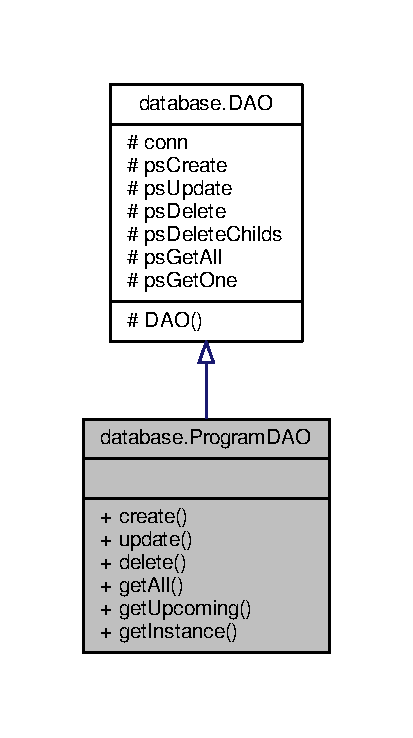
\includegraphics[width=198pt]{classdatabase_1_1ProgramDAO__inherit__graph}
\end{center}
\end{figure}


Collaboration diagram for database.\-Program\-D\-A\-O\-:\nopagebreak
\begin{figure}[H]
\begin{center}
\leavevmode
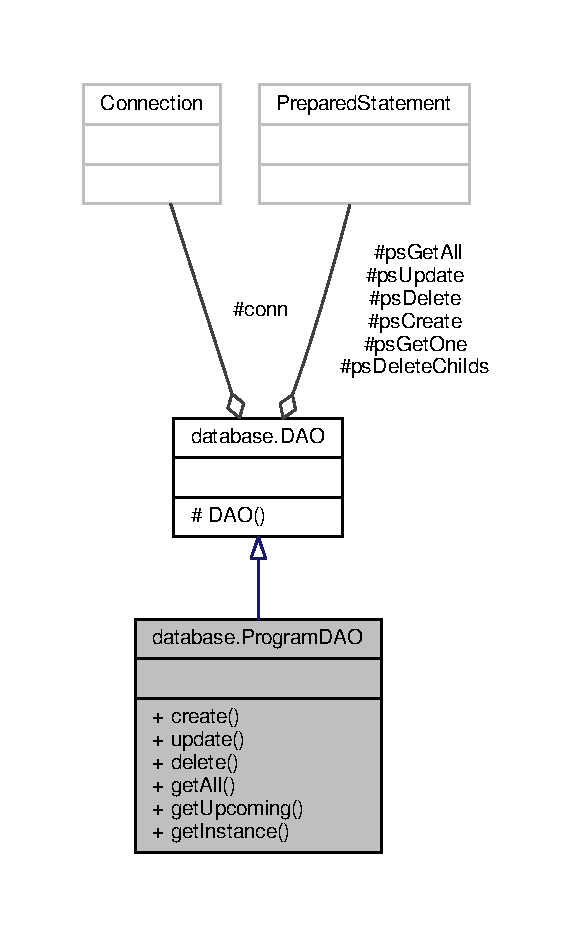
\includegraphics[width=276pt]{classdatabase_1_1ProgramDAO__coll__graph}
\end{center}
\end{figure}
\subsection*{Public Member Functions}
\begin{DoxyCompactItemize}
\item 
void \hyperlink{classdatabase_1_1ProgramDAO_a4b21d41b6f65f50f0d4bbea82b08b3a4}{create} (\hyperlink{classmodel_1_1Program}{Program} program)  throws S\-Q\-L\-Exception 
\begin{DoxyCompactList}\small\item\em Persists new Program. \end{DoxyCompactList}\item 
void \hyperlink{classdatabase_1_1ProgramDAO_a04a0d6682efd0b8de1e4f5a2fb9eff1f}{update} (\hyperlink{classmodel_1_1Program}{Program} program)  throws S\-Q\-L\-Exception 
\begin{DoxyCompactList}\small\item\em Updates Program. \end{DoxyCompactList}\item 
void \hyperlink{classdatabase_1_1ProgramDAO_ad8b438f7c667c619c45fc62c6536b0ec}{delete} (int id)  throws S\-Q\-L\-Exception 
\begin{DoxyCompactList}\small\item\em Deletes Program by I\-D. \end{DoxyCompactList}\item 
Set$<$ \hyperlink{classmodel_1_1Program}{Program} $>$ \hyperlink{classdatabase_1_1ProgramDAO_af130284e455d83524787ab2671eb0325}{get\-All} ()  throws S\-Q\-L\-Exception 
\begin{DoxyCompactList}\small\item\em Gets all Program records from database. \end{DoxyCompactList}\item 
Set$<$ \hyperlink{classmodel_1_1Program}{Program} $>$ \hyperlink{classdatabase_1_1ProgramDAO_a4e35b888111c328029cf2815b95a36a5}{get\-Upcoming} ()  throws S\-Q\-L\-Exception 
\begin{DoxyCompactList}\small\item\em Gets upcoming Program records from database ordered by time. \end{DoxyCompactList}\end{DoxyCompactItemize}
\subsection*{Static Public Member Functions}
\begin{DoxyCompactItemize}
\item 
static \hyperlink{classdatabase_1_1ProgramDAO}{Program\-D\-A\-O} \hyperlink{classdatabase_1_1ProgramDAO_a9b6c7981aee76613fa22242bee6bcfed}{get\-Instance} ()
\begin{DoxyCompactList}\small\item\em Instance getter. \end{DoxyCompactList}\end{DoxyCompactItemize}
\subsection*{Additional Inherited Members}


\subsection{Detailed Description}
\hyperlink{classdatabase_1_1ProgramDAO}{Program\-D\-A\-O} -\/ Data access object for Program 

\begin{DoxyAuthor}{Author}
palmyman 
\end{DoxyAuthor}


\subsection{Member Function Documentation}
\hypertarget{classdatabase_1_1ProgramDAO_a4b21d41b6f65f50f0d4bbea82b08b3a4}{\index{database\-::\-Program\-D\-A\-O@{database\-::\-Program\-D\-A\-O}!create@{create}}
\index{create@{create}!database::ProgramDAO@{database\-::\-Program\-D\-A\-O}}
\subsubsection[{create}]{\setlength{\rightskip}{0pt plus 5cm}void database.\-Program\-D\-A\-O.\-create (
\begin{DoxyParamCaption}
\item[{{\bf Program}}]{program}
\end{DoxyParamCaption}
) throws S\-Q\-L\-Exception\hspace{0.3cm}{\ttfamily [inline]}}}\label{classdatabase_1_1ProgramDAO_a4b21d41b6f65f50f0d4bbea82b08b3a4}


Persists new Program. 


\begin{DoxyParams}{Parameters}
{\em program} & Program to create \\
\hline
\end{DoxyParams}

\begin{DoxyExceptions}{Exceptions}
{\em S\-Q\-L\-Exception} & \\
\hline
\end{DoxyExceptions}
\hypertarget{classdatabase_1_1ProgramDAO_ad8b438f7c667c619c45fc62c6536b0ec}{\index{database\-::\-Program\-D\-A\-O@{database\-::\-Program\-D\-A\-O}!delete@{delete}}
\index{delete@{delete}!database::ProgramDAO@{database\-::\-Program\-D\-A\-O}}
\subsubsection[{delete}]{\setlength{\rightskip}{0pt plus 5cm}void database.\-Program\-D\-A\-O.\-delete (
\begin{DoxyParamCaption}
\item[{int}]{id}
\end{DoxyParamCaption}
) throws S\-Q\-L\-Exception\hspace{0.3cm}{\ttfamily [inline]}}}\label{classdatabase_1_1ProgramDAO_ad8b438f7c667c619c45fc62c6536b0ec}


Deletes Program by I\-D. 


\begin{DoxyParams}{Parameters}
{\em id} & I\-D of Program to delete \\
\hline
\end{DoxyParams}

\begin{DoxyExceptions}{Exceptions}
{\em S\-Q\-L\-Exception} & \\
\hline
\end{DoxyExceptions}
\hypertarget{classdatabase_1_1ProgramDAO_af130284e455d83524787ab2671eb0325}{\index{database\-::\-Program\-D\-A\-O@{database\-::\-Program\-D\-A\-O}!get\-All@{get\-All}}
\index{get\-All@{get\-All}!database::ProgramDAO@{database\-::\-Program\-D\-A\-O}}
\subsubsection[{get\-All}]{\setlength{\rightskip}{0pt plus 5cm}Set$<${\bf Program}$>$ database.\-Program\-D\-A\-O.\-get\-All (
\begin{DoxyParamCaption}
{}
\end{DoxyParamCaption}
) throws S\-Q\-L\-Exception\hspace{0.3cm}{\ttfamily [inline]}}}\label{classdatabase_1_1ProgramDAO_af130284e455d83524787ab2671eb0325}


Gets all Program records from database. 

\begin{DoxyReturn}{Returns}
Set of all Program records from database 
\end{DoxyReturn}

\begin{DoxyExceptions}{Exceptions}
{\em S\-Q\-L\-Exception} & \\
\hline
\end{DoxyExceptions}
\hypertarget{classdatabase_1_1ProgramDAO_a9b6c7981aee76613fa22242bee6bcfed}{\index{database\-::\-Program\-D\-A\-O@{database\-::\-Program\-D\-A\-O}!get\-Instance@{get\-Instance}}
\index{get\-Instance@{get\-Instance}!database::ProgramDAO@{database\-::\-Program\-D\-A\-O}}
\subsubsection[{get\-Instance}]{\setlength{\rightskip}{0pt plus 5cm}static {\bf Program\-D\-A\-O} database.\-Program\-D\-A\-O.\-get\-Instance (
\begin{DoxyParamCaption}
{}
\end{DoxyParamCaption}
)\hspace{0.3cm}{\ttfamily [inline]}, {\ttfamily [static]}}}\label{classdatabase_1_1ProgramDAO_a9b6c7981aee76613fa22242bee6bcfed}


Instance getter. 

\begin{DoxyReturn}{Returns}
instance 
\end{DoxyReturn}
\hypertarget{classdatabase_1_1ProgramDAO_a4e35b888111c328029cf2815b95a36a5}{\index{database\-::\-Program\-D\-A\-O@{database\-::\-Program\-D\-A\-O}!get\-Upcoming@{get\-Upcoming}}
\index{get\-Upcoming@{get\-Upcoming}!database::ProgramDAO@{database\-::\-Program\-D\-A\-O}}
\subsubsection[{get\-Upcoming}]{\setlength{\rightskip}{0pt plus 5cm}Set$<${\bf Program}$>$ database.\-Program\-D\-A\-O.\-get\-Upcoming (
\begin{DoxyParamCaption}
{}
\end{DoxyParamCaption}
) throws S\-Q\-L\-Exception\hspace{0.3cm}{\ttfamily [inline]}}}\label{classdatabase_1_1ProgramDAO_a4e35b888111c328029cf2815b95a36a5}


Gets upcoming Program records from database ordered by time. 

\begin{DoxyReturn}{Returns}
Set of upcoming Program records from database 
\end{DoxyReturn}

\begin{DoxyExceptions}{Exceptions}
{\em S\-Q\-L\-Exception} & \\
\hline
\end{DoxyExceptions}
\hypertarget{classdatabase_1_1ProgramDAO_a04a0d6682efd0b8de1e4f5a2fb9eff1f}{\index{database\-::\-Program\-D\-A\-O@{database\-::\-Program\-D\-A\-O}!update@{update}}
\index{update@{update}!database::ProgramDAO@{database\-::\-Program\-D\-A\-O}}
\subsubsection[{update}]{\setlength{\rightskip}{0pt plus 5cm}void database.\-Program\-D\-A\-O.\-update (
\begin{DoxyParamCaption}
\item[{{\bf Program}}]{program}
\end{DoxyParamCaption}
) throws S\-Q\-L\-Exception\hspace{0.3cm}{\ttfamily [inline]}}}\label{classdatabase_1_1ProgramDAO_a04a0d6682efd0b8de1e4f5a2fb9eff1f}


Updates Program. 


\begin{DoxyParams}{Parameters}
{\em program} & Program to update \\
\hline
\end{DoxyParams}

\begin{DoxyExceptions}{Exceptions}
{\em S\-Q\-L\-Exception} & \\
\hline
\end{DoxyExceptions}


The documentation for this class was generated from the following file\-:\begin{DoxyCompactItemize}
\item 
src/database/Program\-D\-A\-O.\-java\end{DoxyCompactItemize}

\hypertarget{classgui_1_1ProgramEditorDialog}{\section{gui.\-Program\-Editor\-Dialog Class Reference}
\label{classgui_1_1ProgramEditorDialog}\index{gui.\-Program\-Editor\-Dialog@{gui.\-Program\-Editor\-Dialog}}
}


Inheritance diagram for gui.\-Program\-Editor\-Dialog\-:\nopagebreak
\begin{figure}[H]
\begin{center}
\leavevmode
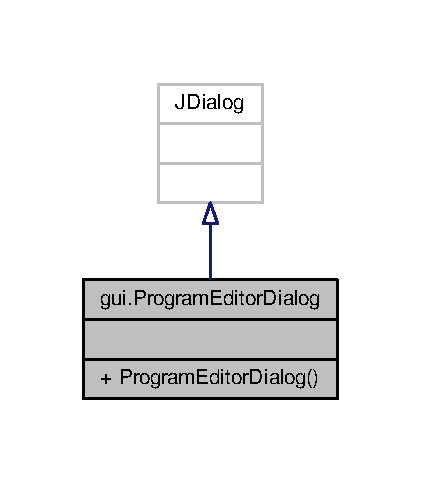
\includegraphics[width=202pt]{classgui_1_1ProgramEditorDialog__inherit__graph}
\end{center}
\end{figure}


Collaboration diagram for gui.\-Program\-Editor\-Dialog\-:\nopagebreak
\begin{figure}[H]
\begin{center}
\leavevmode
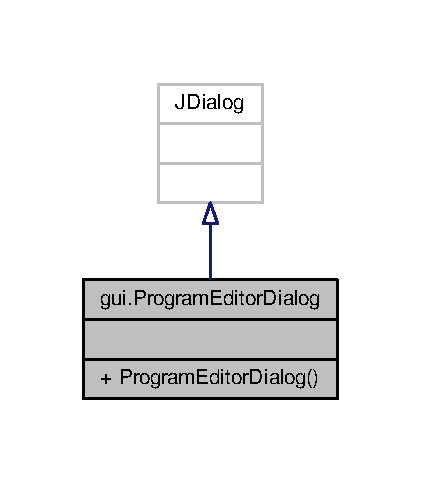
\includegraphics[width=202pt]{classgui_1_1ProgramEditorDialog__coll__graph}
\end{center}
\end{figure}
\subsection*{Public Member Functions}
\begin{DoxyCompactItemize}
\item 
\hypertarget{classgui_1_1ProgramEditorDialog_ad5703137b70b96ad5ef7d3e41ca2da81}{\hyperlink{classgui_1_1ProgramEditorDialog_ad5703137b70b96ad5ef7d3e41ca2da81}{Program\-Editor\-Dialog} ()}\label{classgui_1_1ProgramEditorDialog_ad5703137b70b96ad5ef7d3e41ca2da81}

\begin{DoxyCompactList}\small\item\em Creates new form \hyperlink{classgui_1_1NewProgramDialog}{New\-Program\-Dialog}. \end{DoxyCompactList}\end{DoxyCompactItemize}


\subsection{Detailed Description}
\begin{DoxyAuthor}{Author}
palmyman 
\end{DoxyAuthor}


The documentation for this class was generated from the following file\-:\begin{DoxyCompactItemize}
\item 
src/gui/Program\-Editor\-Dialog.\-java\end{DoxyCompactItemize}

\hypertarget{classservice_1_1Scheduler}{\section{service.\-Scheduler Class Reference}
\label{classservice_1_1Scheduler}\index{service.\-Scheduler@{service.\-Scheduler}}
}


Inheritance diagram for service.\-Scheduler\-:\nopagebreak
\begin{figure}[H]
\begin{center}
\leavevmode
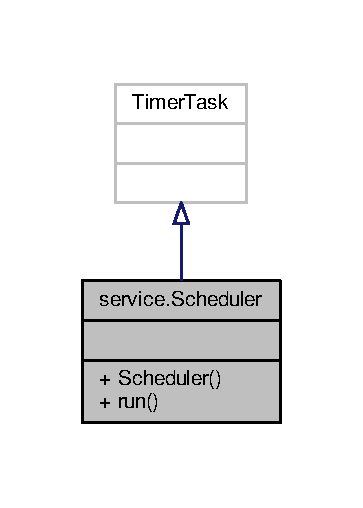
\includegraphics[width=174pt]{classservice_1_1Scheduler__inherit__graph}
\end{center}
\end{figure}


Collaboration diagram for service.\-Scheduler\-:\nopagebreak
\begin{figure}[H]
\begin{center}
\leavevmode
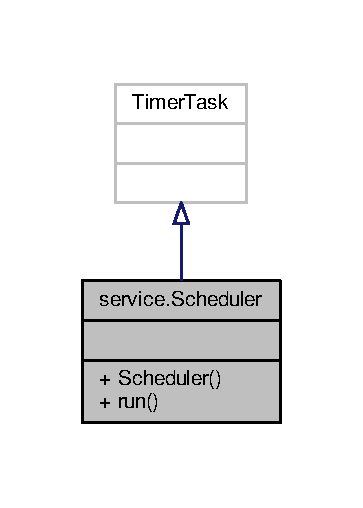
\includegraphics[width=174pt]{classservice_1_1Scheduler__coll__graph}
\end{center}
\end{figure}
\subsection*{Public Member Functions}
\begin{DoxyCompactItemize}
\item 
\hypertarget{classservice_1_1Scheduler_a86fb1f1d344a256e001822082c36362e}{{\bfseries Scheduler} (\hyperlink{classgui_1_1MainFrame}{Main\-Frame} main\-Frame, \hyperlink{classmodel_1_1Program}{Program} program)}\label{classservice_1_1Scheduler_a86fb1f1d344a256e001822082c36362e}

\item 
\hypertarget{classservice_1_1Scheduler_a305649c6c654e1aff685e990d31a9e92}{void {\bfseries run} ()}\label{classservice_1_1Scheduler_a305649c6c654e1aff685e990d31a9e92}

\end{DoxyCompactItemize}


\subsection{Detailed Description}
\begin{DoxyAuthor}{Author}
palmyman 
\end{DoxyAuthor}


The documentation for this class was generated from the following file\-:\begin{DoxyCompactItemize}
\item 
src/service/Scheduler.\-java\end{DoxyCompactItemize}

\hypertarget{classmodel_1_1Sprinkler}{\section{model.\-Sprinkler Class Reference}
\label{classmodel_1_1Sprinkler}\index{model.\-Sprinkler@{model.\-Sprinkler}}
}


Inheritance diagram for model.\-Sprinkler\-:\nopagebreak
\begin{figure}[H]
\begin{center}
\leavevmode
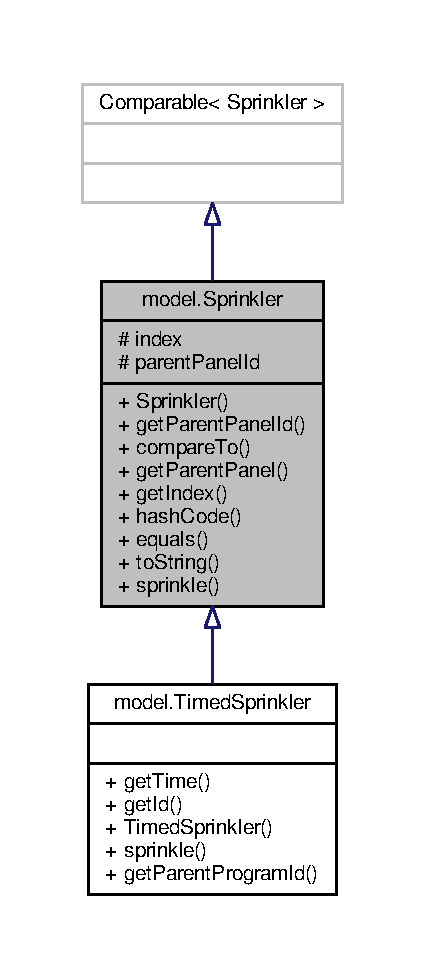
\includegraphics[width=204pt]{classmodel_1_1Sprinkler__inherit__graph}
\end{center}
\end{figure}


Collaboration diagram for model.\-Sprinkler\-:\nopagebreak
\begin{figure}[H]
\begin{center}
\leavevmode
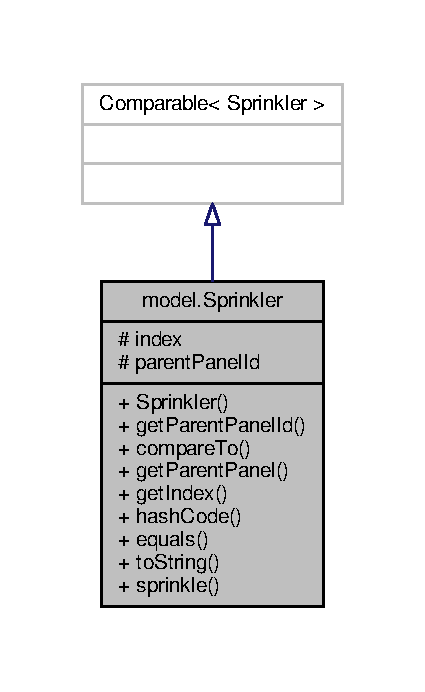
\includegraphics[width=204pt]{classmodel_1_1Sprinkler__coll__graph}
\end{center}
\end{figure}
\subsection*{Public Member Functions}
\begin{DoxyCompactItemize}
\item 
\hyperlink{classmodel_1_1Sprinkler_a126e004e4a7c7be7fa8078c43c77f3f8}{Sprinkler} (int index, int parent\-Panel\-Id)
\item 
int \hyperlink{classmodel_1_1Sprinkler_a24be7eddcf009e4df169e517725127b0}{get\-Parent\-Panel\-Id} ()
\item 
\hypertarget{classmodel_1_1Sprinkler_a413d9983c176f558de511cdae6cc37fb}{int {\bfseries compare\-To} (\hyperlink{classmodel_1_1Sprinkler}{Sprinkler} other)}\label{classmodel_1_1Sprinkler_a413d9983c176f558de511cdae6cc37fb}

\item 
\hyperlink{classmodel_1_1ControlPanel}{Control\-Panel} \hyperlink{classmodel_1_1Sprinkler_ac320304804baa03236250fba2b69197e}{get\-Parent\-Panel} ()
\item 
int \hyperlink{classmodel_1_1Sprinkler_ade1cefff6568e5cbcbbc161235b09d48}{get\-Index} ()
\item 
\hypertarget{classmodel_1_1Sprinkler_a0ed997740b4eba223f93347f2ff02fcf}{int {\bfseries hash\-Code} ()}\label{classmodel_1_1Sprinkler_a0ed997740b4eba223f93347f2ff02fcf}

\item 
\hypertarget{classmodel_1_1Sprinkler_a67629afe3a483e949d969ca29925f049}{boolean {\bfseries equals} (Object obj)}\label{classmodel_1_1Sprinkler_a67629afe3a483e949d969ca29925f049}

\item 
\hypertarget{classmodel_1_1Sprinkler_ad2ada5afb708c8bc737dc36443ff211c}{String {\bfseries to\-String} ()}\label{classmodel_1_1Sprinkler_ad2ada5afb708c8bc737dc36443ff211c}

\item 
void \hyperlink{classmodel_1_1Sprinkler_a44e84feac9ce8ae56f907bb51839bb17}{sprinkle} (int duration)  throws Interrupted\-Exception 
\end{DoxyCompactItemize}
\subsection*{Protected Attributes}
\begin{DoxyCompactItemize}
\item 
\hypertarget{classmodel_1_1Sprinkler_af610d7ff078c5ca794c7246057f629e8}{int {\bfseries index}}\label{classmodel_1_1Sprinkler_af610d7ff078c5ca794c7246057f629e8}

\item 
\hypertarget{classmodel_1_1Sprinkler_abfbc961422b8949e8031ee6eb18da54d}{int {\bfseries parent\-Panel\-Id}}\label{classmodel_1_1Sprinkler_abfbc961422b8949e8031ee6eb18da54d}

\end{DoxyCompactItemize}


\subsection{Detailed Description}
\begin{DoxyAuthor}{Author}
palmyman 
\end{DoxyAuthor}


\subsection{Constructor \& Destructor Documentation}
\hypertarget{classmodel_1_1Sprinkler_a126e004e4a7c7be7fa8078c43c77f3f8}{\index{model\-::\-Sprinkler@{model\-::\-Sprinkler}!Sprinkler@{Sprinkler}}
\index{Sprinkler@{Sprinkler}!model::Sprinkler@{model\-::\-Sprinkler}}
\subsubsection[{Sprinkler}]{\setlength{\rightskip}{0pt plus 5cm}model.\-Sprinkler.\-Sprinkler (
\begin{DoxyParamCaption}
\item[{int}]{index, }
\item[{int}]{parent\-Panel\-Id}
\end{DoxyParamCaption}
)\hspace{0.3cm}{\ttfamily [inline]}}}\label{classmodel_1_1Sprinkler_a126e004e4a7c7be7fa8078c43c77f3f8}

\begin{DoxyParams}{Parameters}
{\em index} & \\
\hline
{\em parent\-Panel\-Id} & \\
\hline
\end{DoxyParams}


\subsection{Member Function Documentation}
\hypertarget{classmodel_1_1Sprinkler_ade1cefff6568e5cbcbbc161235b09d48}{\index{model\-::\-Sprinkler@{model\-::\-Sprinkler}!get\-Index@{get\-Index}}
\index{get\-Index@{get\-Index}!model::Sprinkler@{model\-::\-Sprinkler}}
\subsubsection[{get\-Index}]{\setlength{\rightskip}{0pt plus 5cm}int model.\-Sprinkler.\-get\-Index (
\begin{DoxyParamCaption}
{}
\end{DoxyParamCaption}
)\hspace{0.3cm}{\ttfamily [inline]}}}\label{classmodel_1_1Sprinkler_ade1cefff6568e5cbcbbc161235b09d48}
\begin{DoxyReturn}{Returns}

\end{DoxyReturn}
\hypertarget{classmodel_1_1Sprinkler_ac320304804baa03236250fba2b69197e}{\index{model\-::\-Sprinkler@{model\-::\-Sprinkler}!get\-Parent\-Panel@{get\-Parent\-Panel}}
\index{get\-Parent\-Panel@{get\-Parent\-Panel}!model::Sprinkler@{model\-::\-Sprinkler}}
\subsubsection[{get\-Parent\-Panel}]{\setlength{\rightskip}{0pt plus 5cm}{\bf Control\-Panel} model.\-Sprinkler.\-get\-Parent\-Panel (
\begin{DoxyParamCaption}
{}
\end{DoxyParamCaption}
)\hspace{0.3cm}{\ttfamily [inline]}}}\label{classmodel_1_1Sprinkler_ac320304804baa03236250fba2b69197e}
\begin{DoxyReturn}{Returns}

\end{DoxyReturn}
\hypertarget{classmodel_1_1Sprinkler_a24be7eddcf009e4df169e517725127b0}{\index{model\-::\-Sprinkler@{model\-::\-Sprinkler}!get\-Parent\-Panel\-Id@{get\-Parent\-Panel\-Id}}
\index{get\-Parent\-Panel\-Id@{get\-Parent\-Panel\-Id}!model::Sprinkler@{model\-::\-Sprinkler}}
\subsubsection[{get\-Parent\-Panel\-Id}]{\setlength{\rightskip}{0pt plus 5cm}int model.\-Sprinkler.\-get\-Parent\-Panel\-Id (
\begin{DoxyParamCaption}
{}
\end{DoxyParamCaption}
)\hspace{0.3cm}{\ttfamily [inline]}}}\label{classmodel_1_1Sprinkler_a24be7eddcf009e4df169e517725127b0}
\begin{DoxyReturn}{Returns}

\end{DoxyReturn}
\hypertarget{classmodel_1_1Sprinkler_a44e84feac9ce8ae56f907bb51839bb17}{\index{model\-::\-Sprinkler@{model\-::\-Sprinkler}!sprinkle@{sprinkle}}
\index{sprinkle@{sprinkle}!model::Sprinkler@{model\-::\-Sprinkler}}
\subsubsection[{sprinkle}]{\setlength{\rightskip}{0pt plus 5cm}void model.\-Sprinkler.\-sprinkle (
\begin{DoxyParamCaption}
\item[{int}]{duration}
\end{DoxyParamCaption}
) throws Interrupted\-Exception\hspace{0.3cm}{\ttfamily [inline]}}}\label{classmodel_1_1Sprinkler_a44e84feac9ce8ae56f907bb51839bb17}

\begin{DoxyParams}{Parameters}
{\em duration} & \\
\hline
\end{DoxyParams}

\begin{DoxyExceptions}{Exceptions}
{\em Interrupted\-Exception} & \\
\hline
\end{DoxyExceptions}


The documentation for this class was generated from the following file\-:\begin{DoxyCompactItemize}
\item 
src/model/Sprinkler.\-java\end{DoxyCompactItemize}

\hypertarget{classdatabase_1_1SprinklerDAO}{\section{database.\-Sprinkler\-D\-A\-O Class Reference}
\label{classdatabase_1_1SprinklerDAO}\index{database.\-Sprinkler\-D\-A\-O@{database.\-Sprinkler\-D\-A\-O}}
}


\hyperlink{classdatabase_1_1SprinklerDAO}{Sprinkler\-D\-A\-O} -\/ Data access object for Sprinkler  




Inheritance diagram for database.\-Sprinkler\-D\-A\-O\-:\nopagebreak
\begin{figure}[H]
\begin{center}
\leavevmode
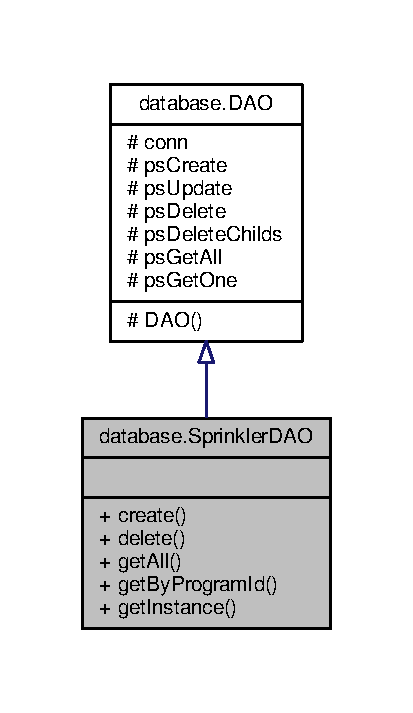
\includegraphics[width=198pt]{classdatabase_1_1SprinklerDAO__inherit__graph}
\end{center}
\end{figure}


Collaboration diagram for database.\-Sprinkler\-D\-A\-O\-:\nopagebreak
\begin{figure}[H]
\begin{center}
\leavevmode
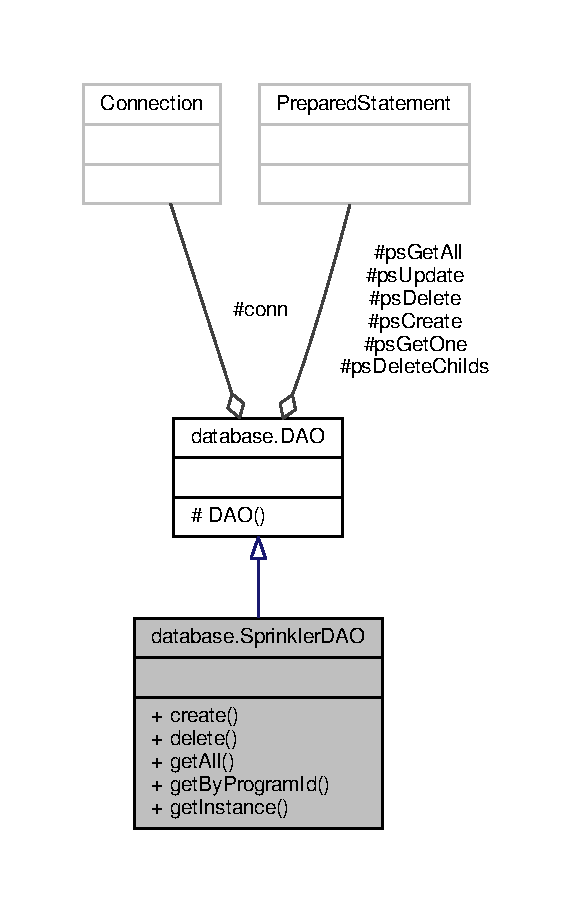
\includegraphics[width=276pt]{classdatabase_1_1SprinklerDAO__coll__graph}
\end{center}
\end{figure}
\subsection*{Public Member Functions}
\begin{DoxyCompactItemize}
\item 
void \hyperlink{classdatabase_1_1SprinklerDAO_aa36660d2b73caa79fa7ad6f85cdf5d73}{create} (\hyperlink{classmodel_1_1TimedSprinkler}{Timed\-Sprinkler} sprinkler)  throws S\-Q\-L\-Exception 
\begin{DoxyCompactList}\small\item\em Persists new Timed\-Sprinkler. \end{DoxyCompactList}\item 
void \hyperlink{classdatabase_1_1SprinklerDAO_a9fa3398276c78b71f4e35a54085515c7}{delete} (int id)  throws S\-Q\-L\-Exception 
\begin{DoxyCompactList}\small\item\em Deletes Timed\-Sprinkler from database by I\-D. \end{DoxyCompactList}\item 
Set$<$ \hyperlink{classmodel_1_1TimedSprinkler}{Timed\-Sprinkler} $>$ \hyperlink{classdatabase_1_1SprinklerDAO_ada482a94d720543499345f7431665875}{get\-All} ()  throws S\-Q\-L\-Exception 
\begin{DoxyCompactList}\small\item\em Gets all Timed\-Sprinklers from database. \end{DoxyCompactList}\item 
Set$<$ \hyperlink{classmodel_1_1TimedSprinkler}{Timed\-Sprinkler} $>$ \hyperlink{classdatabase_1_1SprinklerDAO_a89a1aee06da7613937d4f2b8b482d65f}{get\-By\-Program\-Id} (int program\-Id)  throws S\-Q\-L\-Exception 
\begin{DoxyCompactList}\small\item\em Gets Timed\-Sprinklers by Program I\-D. \end{DoxyCompactList}\end{DoxyCompactItemize}
\subsection*{Static Public Member Functions}
\begin{DoxyCompactItemize}
\item 
static \hyperlink{classdatabase_1_1SprinklerDAO}{Sprinkler\-D\-A\-O} \hyperlink{classdatabase_1_1SprinklerDAO_a1437d73a7864607e52b923af135227d0}{get\-Instance} ()
\begin{DoxyCompactList}\small\item\em Instance getter. \end{DoxyCompactList}\end{DoxyCompactItemize}
\subsection*{Additional Inherited Members}


\subsection{Detailed Description}
\hyperlink{classdatabase_1_1SprinklerDAO}{Sprinkler\-D\-A\-O} -\/ Data access object for Sprinkler 

\begin{DoxyAuthor}{Author}
palmyman 
\end{DoxyAuthor}


\subsection{Member Function Documentation}
\hypertarget{classdatabase_1_1SprinklerDAO_aa36660d2b73caa79fa7ad6f85cdf5d73}{\index{database\-::\-Sprinkler\-D\-A\-O@{database\-::\-Sprinkler\-D\-A\-O}!create@{create}}
\index{create@{create}!database::SprinklerDAO@{database\-::\-Sprinkler\-D\-A\-O}}
\subsubsection[{create}]{\setlength{\rightskip}{0pt plus 5cm}void database.\-Sprinkler\-D\-A\-O.\-create (
\begin{DoxyParamCaption}
\item[{{\bf Timed\-Sprinkler}}]{sprinkler}
\end{DoxyParamCaption}
) throws S\-Q\-L\-Exception\hspace{0.3cm}{\ttfamily [inline]}}}\label{classdatabase_1_1SprinklerDAO_aa36660d2b73caa79fa7ad6f85cdf5d73}


Persists new Timed\-Sprinkler. 


\begin{DoxyParams}{Parameters}
{\em sprinkler} & Timed\-Sprinkler to persist \\
\hline
\end{DoxyParams}

\begin{DoxyExceptions}{Exceptions}
{\em S\-Q\-L\-Exception} & \\
\hline
\end{DoxyExceptions}
\hypertarget{classdatabase_1_1SprinklerDAO_a9fa3398276c78b71f4e35a54085515c7}{\index{database\-::\-Sprinkler\-D\-A\-O@{database\-::\-Sprinkler\-D\-A\-O}!delete@{delete}}
\index{delete@{delete}!database::SprinklerDAO@{database\-::\-Sprinkler\-D\-A\-O}}
\subsubsection[{delete}]{\setlength{\rightskip}{0pt plus 5cm}void database.\-Sprinkler\-D\-A\-O.\-delete (
\begin{DoxyParamCaption}
\item[{int}]{id}
\end{DoxyParamCaption}
) throws S\-Q\-L\-Exception\hspace{0.3cm}{\ttfamily [inline]}}}\label{classdatabase_1_1SprinklerDAO_a9fa3398276c78b71f4e35a54085515c7}


Deletes Timed\-Sprinkler from database by I\-D. 


\begin{DoxyParams}{Parameters}
{\em id} & I\-D of Timed\-Sprinkler to delete \\
\hline
\end{DoxyParams}

\begin{DoxyExceptions}{Exceptions}
{\em S\-Q\-L\-Exception} & \\
\hline
\end{DoxyExceptions}
\hypertarget{classdatabase_1_1SprinklerDAO_ada482a94d720543499345f7431665875}{\index{database\-::\-Sprinkler\-D\-A\-O@{database\-::\-Sprinkler\-D\-A\-O}!get\-All@{get\-All}}
\index{get\-All@{get\-All}!database::SprinklerDAO@{database\-::\-Sprinkler\-D\-A\-O}}
\subsubsection[{get\-All}]{\setlength{\rightskip}{0pt plus 5cm}Set$<${\bf Timed\-Sprinkler}$>$ database.\-Sprinkler\-D\-A\-O.\-get\-All (
\begin{DoxyParamCaption}
{}
\end{DoxyParamCaption}
) throws S\-Q\-L\-Exception\hspace{0.3cm}{\ttfamily [inline]}}}\label{classdatabase_1_1SprinklerDAO_ada482a94d720543499345f7431665875}


Gets all Timed\-Sprinklers from database. 

\begin{DoxyReturn}{Returns}
Set of all Timed\-Sprinklers 
\end{DoxyReturn}

\begin{DoxyExceptions}{Exceptions}
{\em S\-Q\-L\-Exception} & \\
\hline
\end{DoxyExceptions}
\hypertarget{classdatabase_1_1SprinklerDAO_a89a1aee06da7613937d4f2b8b482d65f}{\index{database\-::\-Sprinkler\-D\-A\-O@{database\-::\-Sprinkler\-D\-A\-O}!get\-By\-Program\-Id@{get\-By\-Program\-Id}}
\index{get\-By\-Program\-Id@{get\-By\-Program\-Id}!database::SprinklerDAO@{database\-::\-Sprinkler\-D\-A\-O}}
\subsubsection[{get\-By\-Program\-Id}]{\setlength{\rightskip}{0pt plus 5cm}Set$<${\bf Timed\-Sprinkler}$>$ database.\-Sprinkler\-D\-A\-O.\-get\-By\-Program\-Id (
\begin{DoxyParamCaption}
\item[{int}]{program\-Id}
\end{DoxyParamCaption}
) throws S\-Q\-L\-Exception\hspace{0.3cm}{\ttfamily [inline]}}}\label{classdatabase_1_1SprinklerDAO_a89a1aee06da7613937d4f2b8b482d65f}


Gets Timed\-Sprinklers by Program I\-D. 


\begin{DoxyParams}{Parameters}
{\em program\-Id} & I\-D of planed Program \\
\hline
\end{DoxyParams}
\begin{DoxyReturn}{Returns}
Set of Timed\-Sprinklers planed in Program 
\end{DoxyReturn}

\begin{DoxyExceptions}{Exceptions}
{\em S\-Q\-L\-Exception} & \\
\hline
\end{DoxyExceptions}
\hypertarget{classdatabase_1_1SprinklerDAO_a1437d73a7864607e52b923af135227d0}{\index{database\-::\-Sprinkler\-D\-A\-O@{database\-::\-Sprinkler\-D\-A\-O}!get\-Instance@{get\-Instance}}
\index{get\-Instance@{get\-Instance}!database::SprinklerDAO@{database\-::\-Sprinkler\-D\-A\-O}}
\subsubsection[{get\-Instance}]{\setlength{\rightskip}{0pt plus 5cm}static {\bf Sprinkler\-D\-A\-O} database.\-Sprinkler\-D\-A\-O.\-get\-Instance (
\begin{DoxyParamCaption}
{}
\end{DoxyParamCaption}
)\hspace{0.3cm}{\ttfamily [inline]}, {\ttfamily [static]}}}\label{classdatabase_1_1SprinklerDAO_a1437d73a7864607e52b923af135227d0}


Instance getter. 

\begin{DoxyReturn}{Returns}
instance 
\end{DoxyReturn}


The documentation for this class was generated from the following file\-:\begin{DoxyCompactItemize}
\item 
src/database/Sprinkler\-D\-A\-O.\-java\end{DoxyCompactItemize}

\hypertarget{classmodel_1_1TimedSprinkler}{\section{model.\-Timed\-Sprinkler Class Reference}
\label{classmodel_1_1TimedSprinkler}\index{model.\-Timed\-Sprinkler@{model.\-Timed\-Sprinkler}}
}


Inheritance diagram for model.\-Timed\-Sprinkler\-:\nopagebreak
\begin{figure}[H]
\begin{center}
\leavevmode
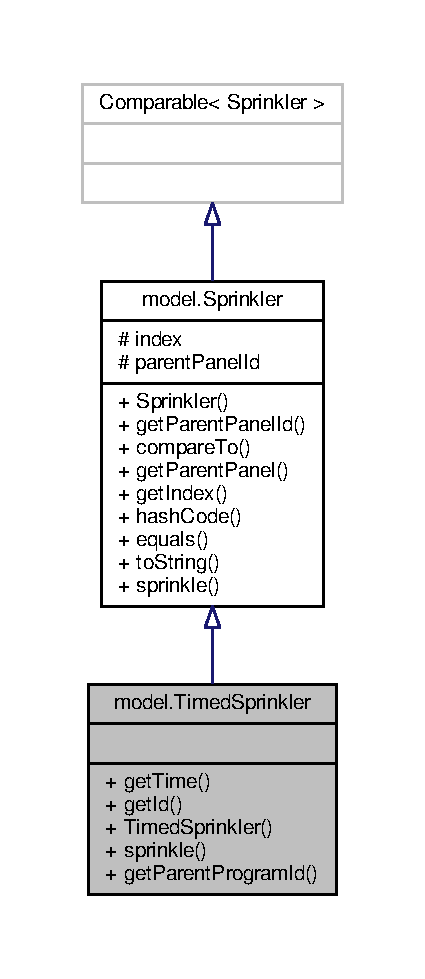
\includegraphics[width=204pt]{classmodel_1_1TimedSprinkler__inherit__graph}
\end{center}
\end{figure}


Collaboration diagram for model.\-Timed\-Sprinkler\-:\nopagebreak
\begin{figure}[H]
\begin{center}
\leavevmode
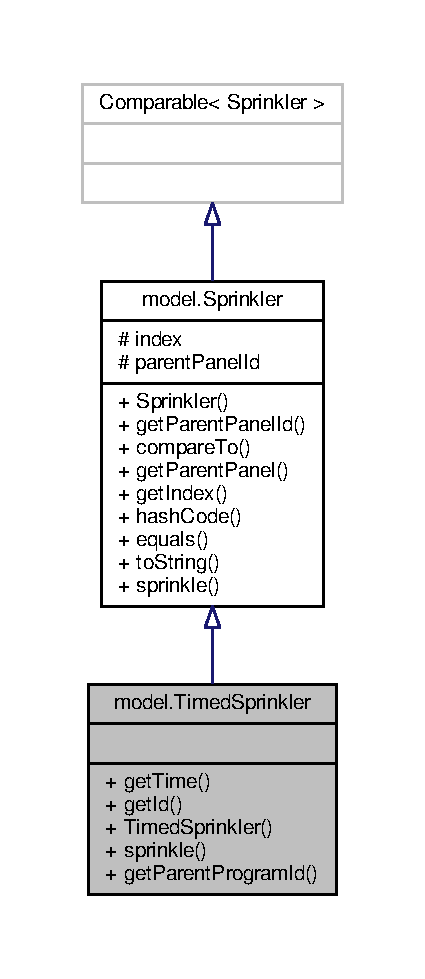
\includegraphics[width=204pt]{classmodel_1_1TimedSprinkler__coll__graph}
\end{center}
\end{figure}
\subsection*{Public Member Functions}
\begin{DoxyCompactItemize}
\item 
int \hyperlink{classmodel_1_1TimedSprinkler_ab0ba114252c55ec7995d58376750485a}{get\-Time} ()
\item 
int \hyperlink{classmodel_1_1TimedSprinkler_aaf2924a2f3e51954bcbdf2221ca6a4aa}{get\-Id} ()
\item 
\hyperlink{classmodel_1_1TimedSprinkler_ae55b6aac3c65f6962911ef91bf3d8aee}{Timed\-Sprinkler} (\hyperlink{classmodel_1_1Sprinkler}{Sprinkler} sprinkler, int id, int patent\-Program\-Id, int time)
\item 
void \hyperlink{classmodel_1_1TimedSprinkler_a2c48212b71d77beff3442ed76fede2d9}{sprinkle} ()  throws Interrupted\-Exception 
\item 
int \hyperlink{classmodel_1_1TimedSprinkler_a497ab6c4dd45f3d217084745d988d901}{get\-Parent\-Program\-Id} ()
\end{DoxyCompactItemize}
\subsection*{Additional Inherited Members}


\subsection{Detailed Description}
\begin{DoxyAuthor}{Author}
palmyman 
\end{DoxyAuthor}


\subsection{Constructor \& Destructor Documentation}
\hypertarget{classmodel_1_1TimedSprinkler_ae55b6aac3c65f6962911ef91bf3d8aee}{\index{model\-::\-Timed\-Sprinkler@{model\-::\-Timed\-Sprinkler}!Timed\-Sprinkler@{Timed\-Sprinkler}}
\index{Timed\-Sprinkler@{Timed\-Sprinkler}!model::TimedSprinkler@{model\-::\-Timed\-Sprinkler}}
\subsubsection[{Timed\-Sprinkler}]{\setlength{\rightskip}{0pt plus 5cm}model.\-Timed\-Sprinkler.\-Timed\-Sprinkler (
\begin{DoxyParamCaption}
\item[{{\bf Sprinkler}}]{sprinkler, }
\item[{int}]{id, }
\item[{int}]{patent\-Program\-Id, }
\item[{int}]{time}
\end{DoxyParamCaption}
)\hspace{0.3cm}{\ttfamily [inline]}}}\label{classmodel_1_1TimedSprinkler_ae55b6aac3c65f6962911ef91bf3d8aee}

\begin{DoxyParams}{Parameters}
{\em sprinkler} & \\
\hline
{\em id} & \\
\hline
{\em patent\-Program\-Id} & \\
\hline
{\em time} & \\
\hline
\end{DoxyParams}


\subsection{Member Function Documentation}
\hypertarget{classmodel_1_1TimedSprinkler_aaf2924a2f3e51954bcbdf2221ca6a4aa}{\index{model\-::\-Timed\-Sprinkler@{model\-::\-Timed\-Sprinkler}!get\-Id@{get\-Id}}
\index{get\-Id@{get\-Id}!model::TimedSprinkler@{model\-::\-Timed\-Sprinkler}}
\subsubsection[{get\-Id}]{\setlength{\rightskip}{0pt plus 5cm}int model.\-Timed\-Sprinkler.\-get\-Id (
\begin{DoxyParamCaption}
{}
\end{DoxyParamCaption}
)\hspace{0.3cm}{\ttfamily [inline]}}}\label{classmodel_1_1TimedSprinkler_aaf2924a2f3e51954bcbdf2221ca6a4aa}
\begin{DoxyReturn}{Returns}

\end{DoxyReturn}
\hypertarget{classmodel_1_1TimedSprinkler_a497ab6c4dd45f3d217084745d988d901}{\index{model\-::\-Timed\-Sprinkler@{model\-::\-Timed\-Sprinkler}!get\-Parent\-Program\-Id@{get\-Parent\-Program\-Id}}
\index{get\-Parent\-Program\-Id@{get\-Parent\-Program\-Id}!model::TimedSprinkler@{model\-::\-Timed\-Sprinkler}}
\subsubsection[{get\-Parent\-Program\-Id}]{\setlength{\rightskip}{0pt plus 5cm}int model.\-Timed\-Sprinkler.\-get\-Parent\-Program\-Id (
\begin{DoxyParamCaption}
{}
\end{DoxyParamCaption}
)\hspace{0.3cm}{\ttfamily [inline]}}}\label{classmodel_1_1TimedSprinkler_a497ab6c4dd45f3d217084745d988d901}
\begin{DoxyReturn}{Returns}

\end{DoxyReturn}
\hypertarget{classmodel_1_1TimedSprinkler_ab0ba114252c55ec7995d58376750485a}{\index{model\-::\-Timed\-Sprinkler@{model\-::\-Timed\-Sprinkler}!get\-Time@{get\-Time}}
\index{get\-Time@{get\-Time}!model::TimedSprinkler@{model\-::\-Timed\-Sprinkler}}
\subsubsection[{get\-Time}]{\setlength{\rightskip}{0pt plus 5cm}int model.\-Timed\-Sprinkler.\-get\-Time (
\begin{DoxyParamCaption}
{}
\end{DoxyParamCaption}
)\hspace{0.3cm}{\ttfamily [inline]}}}\label{classmodel_1_1TimedSprinkler_ab0ba114252c55ec7995d58376750485a}
\begin{DoxyReturn}{Returns}

\end{DoxyReturn}
\hypertarget{classmodel_1_1TimedSprinkler_a2c48212b71d77beff3442ed76fede2d9}{\index{model\-::\-Timed\-Sprinkler@{model\-::\-Timed\-Sprinkler}!sprinkle@{sprinkle}}
\index{sprinkle@{sprinkle}!model::TimedSprinkler@{model\-::\-Timed\-Sprinkler}}
\subsubsection[{sprinkle}]{\setlength{\rightskip}{0pt plus 5cm}void model.\-Timed\-Sprinkler.\-sprinkle (
\begin{DoxyParamCaption}
{}
\end{DoxyParamCaption}
) throws Interrupted\-Exception\hspace{0.3cm}{\ttfamily [inline]}}}\label{classmodel_1_1TimedSprinkler_a2c48212b71d77beff3442ed76fede2d9}

\begin{DoxyExceptions}{Exceptions}
{\em Interrupted\-Exception} & \\
\hline
\end{DoxyExceptions}


The documentation for this class was generated from the following file\-:\begin{DoxyCompactItemize}
\item 
src/model/Timed\-Sprinkler.\-java\end{DoxyCompactItemize}

%--- End generated contents ---

% Index
\newpage
\phantomsection
\addcontentsline{toc}{chapter}{Index}
\printindex

\end{document}
